% Force internal link target to this chapter
% Reference page from javadoc via <a href="/doc/duccbook.html#DUCC_CLI">whatever text</a>
\ifpdf
\else
\HCode{<a name='DUCC_CLI'></a>}
\fi
\chapter{Command Line Interface}
\label{chap:cli}

    \paragraph{The DUCC Job Descriptor}
    The DUCC Job Descriptor includes properties to enable automated management and scale-out 
    over large computing clusters.  The job descriptor includes
    \begin{itemize}
      \item References to the various UIMA components required by the job (CR, CM, AE, CC, and maybe DD)
      \item Scale-out requirements: number of processes, number of threads per process, etc
      \item Environment requirments: log directory, working directory, environment variables, etc,
      \item JVM paramenters
      \item Scheduling class
      \item Error-handling preferences: acceptable failure counts, timeouts, etc
      \item Debugging and monitoring requirements and preferences
    \end{itemize}
  

    The Command Line Interface is provided in several forms:

    \begin{enumerate}
      \item A Java executable jar.
      \item A script.
      \item Direct invocation of each commands's {\tt main}.
    \end{enumerate}

    When using the executable jars and scripts the full execution environment is estableshed
    silently.  When directly invoking a command's {\tt main} one must set the java {\tt CLASSPATH} to
    specify the appropriate jar for the command, as described in subsequent sections.

    The following commands are provided:
    \begin{description}
    \item[ducc\_submit] Submit a job for ececution.
    \item[ducc\_cancel] Cancel a job in progress.
    \item[ducc\_reserve] Request a reservation of full or partial machines.
    \item[ducc\_unreserve] Cancel a reservation.
    \item[ducc\_monitor] Monitor the progress of a job that is already submitted.
    \item[ducc\_process\_submit] Submit an arbitrary process (managed reservation) for execution.
    \item[ducc\_process\_cancel] Cancel an arbitrary process.
    \item[ducc\_service\_submit] Submit a (non-registered) service instance for execution.
    \item[ducc\_service\_cancel] Cancel a (non-registered) service instance.
    \item[ducc\_services] Register, unregister, start, stop, modify, and query a service.
    \end{description}
    
    The next section describes these commands in detail.

    %% These all input sections
    % Create well-known link to this spot for HTML version
\ifpdf
\else
\HCode{<a name='DUCC_CLI_SUBMIT'></a>}
\fi

    \section{ducc\_submit}
    \label{sec:cli.ducc-submit}
       The source for this section is ducc\_duccbook/documents/part-user/cli/submit.xml.
       \paragraph{Description:}
           The submit CLI is used to submit work for execution by DUCC. DUCC assigns a unique id to the
           job and schedules it for execution. The submitter may optionally request that the progress of
           the job is monitored, in which case the state of the job as it progresses through its
           lifetime is printed on the console.
       \paragraph{Usage:}
           \begin{description}
             \item[Script wrapper] \ducchome/bin/ducc\_submit {\em options}
             \item[Java Main]      java -cp \ducchome/lib/uima-ducc-cli.jar org.apache.uima.ducc.cli.DuccJobSubmit {\em options}
           \end{description}

        \paragraph{Options:}
           \begin{description}

           \item[$--$all\_in\_one $<$local $|$ remote $>$]
               Run driver and pipeline in single process.  If {\em local} is specified, the
               process is executed on the local machine, for example, in the current Eclipse session.
               If {\em remote} is specified, the jobs is submitted to DUCC as a {\em manged reservation}
               and run on some (presumably larger) machine allocated by DUCC.

           \item[$--$attach\_console] If specified, redirect remote stdout and stderr
             to the local submitting console.

           \item[$--$cancel\_on\_interrupt].  If the job is started with $--$wait\_for\_completion, this
             option causes the job to be canceled if the submit command is terminated,
             e.g., with CTL-C. If $--$cancel\_job\_on\_interrupt is not
             specified, the job monitor will be terminated but the job will continue to run.

             If $--$wait\_for\_completion is not specified this option is ignored. 

           \item[$--$classpath] The CLASSPATH used for the job.  If specified, this is used
             for both the Job Driver and each Job Process. If not specified the CLASSPATH found by the underlying
             {\tt DuccJobSubmit.main()} method is used.

           \item[$--$classpath\_order {[user-before-ducc $|$ ducc-before-user]} ]
             When DUCC deploys a process, set the user-supplied CLASSPATH before DUCC-supplied
             CLASSPATH, or the reverse. The default is user-before-ducc.
             
           \item[$--$debug] Enable debugging messages. This is primarily for debugging DUCC itself.

           \item[$--$description {[text]}] The text is any string used to describe the job. It is
             displayed in the Web Server. When specified on a command-line the text usually 
             must be surrounded by quotes to protect it from the shell.  The default is ``none''.

           \item[$--$attach\_console] If specified, redirect remote stdout and stderr
             to the local submitting console.

           \item[$--$driver\_debug {[debugger-address]}] Append JVM debug flags to the JVM arguments
             to start the JobDriver in remote debug mode.  The remote process debugger will attempt
             to contact the specified port. The address is of the form {\tt host:port}.

           \item[$--$driver\_descriptor\_CR {[descriptor.xml]} ] This is the XML descriptor for the
             Collection Reader.  This descriptor is a resource that is searched for in the CLASSPATH
             and data path as described in the ~\hyperref[par:cli.submit.notes]{notes below}.

           \item[$--$driver\_descriptor\_CR\_overrides {[list]} ]             
             This is the Job Driver collection reader configuration overrides. They are specified as 
             name/value pairs in a comma-delimited list. For example: 
             \begin{verbatim}
--driver_descriptor_CR_overrides name1=value1,name2=value2...
             \end{verbatim}
             
             
%           \item[$--$driver\_environment {[list]} ]
%
%             This specifies environment parameters for the Job Driver. If present, they are added to the 
%             Job Driver's environment as the process is spawned. It must be a quoted, blank-delimeted 
%             lsit of name-value pairs. For example: 
%             \begin{verbatim}
%"TERM=xterm DISPLAY=:1.0" 
%             \end{verbatim}
%             
%             Note: On Secure Linux systems, the environemnt variable 
%             LD\_LIBRARY\_PATH may not be passed to the user's program. If it is 
%             necessary to pass LD\_LIBRARY\_PATH to the JP or JD processes, it must be 
%             specified as DUCC\_LD\_LIBRARY\_PATH. Ducc (securely) passes this as 
%             LD\_LIBRARY\_PATH, after the JP or JD has assumed the user's identity. For 
%             example: 
%             \begin{verbatim}
%"--process\_environment TERM=xterm DISPLAY=:1.0 DUCC\_LD\_LIBRARY\_PATH=/my/own/
%            \end{verbatim}

           \item[$--$driver\_exception\_handler {[classname]}] This specifies a developer-supplied
             exception handler for the Job Driver.  It must
             implement org.apache.uima.ducc.common.jd.plugin.IJdProcessExceptionHandler or extend
             org.apache.uima.ducc.common.jd.plugin.AbstractJdProcessExceptionHandler.  A default
             handler is provided.


           \item[$--$driver\_jvm\_args {[list]} ]

             This specifies extra JVM arguments to be provided to the Job Driver process. It is a blank delimited 
             list of strings. Example: 
             \begin{verbatim}
--driver_jvm_args -Xmx100M -Xms50M 
             \end{verbatim}

             Note: When used as a CLI option, the list must usually be
             quoted to protect it from the shell.
             
           \item[$--$environment {[env vars]}] Blank-delimited list of environment variable
             assignments. If specified, this is used for all DUCC processes in the job. Example:
             \begin{verbatim}
--environment TERM=xterm DISPLAY=:1.0
             \end{verbatim}
             
             Additional entries may be copied from the user's environment based on the setting of
             ducc.submit.environment.propagated in the global DUCC configuration ducc.properties.

             Note: When used as a CLI option, the environment string must usually be
             quoted to protect it from the shell.

           \item[$--$help ]

             Prints the usage text to the console. 

           \item[$--$jvm {[path-to-java]}  ]

             States the JVM to use. If not specified, the same JVM used by the Agents is used.  This is
             the full path to the JVM, not the JAVA\_HOME.
             Example: 
\begin{verbatim}
--jvm /share/jdk1.6/bin/java 
\end{verbatim}
             
           \item[$--$log\_directory {[path-to-log-directory]} ]

             This specifies the path to the directory for the user logs. If not specified, the default is
             \$HOME/ducc/logs. Example: 
             \begin{verbatim}
--log_directory /home/bob 
             \end{verbatim}
             
             Within this directory DUCC creates a sub-directory for each job, using the unique numerical 
             ID of the job. The format of the generated log file names as described
             \hyperref[chap:job-logs]{here}.
             
             Note: Note that $--$log\_directory specifies only the path to a directory where 
             logs are to be stored. In order to manage multiple processes running in multiple 
             machines, sub-directory and file names are generated by DUCC and may 
             not be directly specified. 

           \item[$--$process\_DD {[DD descriptor]}  ]

             This specifies a UIMA Deployment Descriptor for the job processes for DD-style jobs. 
             This is mutually exclusive with $--$process\_descriptor\_AE, $--$process\_descriptor\_CM, 
             and $--$process\_descriptor\_CC. This descriptor is a resource that is searched for in the 
             CLASSPATH and data path as described in the ~\hyperref[par:cli.submit.notes]{notes below}.
             For example:
             \begin{verbatim}
--process_DD /home/billy/resource/DD_foo.xml 
             \end{verbatim}

           \item[$--$process\_debug {[debugger-address]}] Append JVM debug flags to the JVM
             arguments to start the Job Process in remote debug mode.  The remote process will start
             its debugger and attempt to contact the debugger (usually Eclipse) on the specified
             port.  The address is of the form {\tt host:port}.
             
           \item[$--$process\_deployments\_max {[integer]} ]

             This specifies the maximum number of Job Processes to deploy at any given time. If not 
             specified, DUCC will attempt to provide the largest number of processes within the 
             constraints of fair\_share scheduling and the amount of work remaining.
             in the job. Example:
             \begin{verbatim}
--process_deployments_max 66 
             \end{verbatim}


           \item[$--$process\_descriptor\_AE {[descriptor]}  ]

             This specifies the Analysis Engine descriptor to be deployed in the Job Processes. This 
             descriptor is a resource that is searched for in the CLASSPATH and data path as described 
             in the ~\hyperref[par:cli.submit.notes]{notes below}.
             It is mutually exclusive with $--$process\_DD For example: 
             \begin{verbatim}
--process_descriptor_AE /home/billy/resource/AE_foo.xml 
             \end{verbatim}


           \item[$--$process\_descriptor\_AE\_overrides {[list]}  ]

             This specifies AE overrides. It is a comma-delimited list of name/value pairs. Example: 
             \begin{verbatim}
--process_descriptor_AE_Overrides name1=value1,name2=value2 
             \end{verbatim}
             
           \item[$--$process\_descriptor\_CC {[descriptor]}  ]

             This specifies the CAS Consumer descriptor to be deployed in the Job Processes. This 
             descriptor is a resource that is searched for in the CLASSPATH and data path as described 
             in the ~\hyperref[par:cli.submit.notes]{notes below}.
             It is mutually exclusive with $--$process\_DD For example: 
             \begin{verbatim}
--process_descriptor_CC /home/billy/resourceCCE_foo.xml 
             \end{verbatim}
             
           \item[$--$process\_descriptor\_CC\_overrides {[list]}  ]

             This specifies CC overrides. It is a comma-delimited list of name/value pairs. Example: 
             \begin{verbatim}
--process_descriptor_CC_overrides name1=value1,name2=value2 
             \end{verbatim}
             
           \item[$--$process\_descriptor\_CM {[descriptor]} ]

             This specifies the CAS Multiplier descriptor to be deployed in the Job Processes. This 
             descriptor is a resource that is searched for in the CLASSPATH and data path as described 
             in the ~\hyperref[par:cli.submit.notes]{notes below}.
             It is mutually exclusive with $--$process\_DD For example: 
             \begin{verbatim}             
--process_descriptor_CM /home/billy/resource/CM_foo.xml 
             \end{verbatim}

           \item[$--$process\_descriptor\_CM\_overrides {[list]}  ]

             This specifies CM overrides. It is a comma-delimited list of name/value pairs. Example: 
             \begin{verbatim}
--process_descriptor_CM_overrides name1=value1,name2=value2 
\end{verbatim}
             
           \item[$--$process\_failures\_limit {[integer]} ]

             This specifies the maximum number of individual Job Process (JP) failures allowed
             before killing the job. The default is fifteen(15). If this limit is exceeded over the lifetime 
             of a job DUCC terminates the entire job. 
             \begin{verbatim}
--process_failures_limit 23
\end{verbatim}
                          
           \item[$--$process\_initialization\_failures\_cap {[integer]} ] This specifies the maximum
             number of failures during a UIMA process's initialization phase.  If the number is
             exceeded the system will allow processes which are already running to continue, but
             will assign no new processes to the job.  The default is ninety-nine(99). Example:
             \begin{verbatim}
--process_initialization_failures_cap 62 
             \end{verbatim}
             
             Note that the job is NOT killed if there are processes that have passed initialization and are 
             running. If this limit is reached, the only action is to not start new processes for the job. 

           \item[$--$process\_initialization\_time\_max {[integer]}] This is the maximum time a process
             is allowed to remain in the ``initializing'' state, before DUCC terminates it.  The error
             counts as an initialization error towards the initialization failure cap.

           \item[$--$process\_jvm\_args {[list]} ] This specifies additional arguments to be passed to
             the Job Process JVM as a blank-delimited list of strings. Example:
             \begin{verbatim}
--process_jvm_args -Xmx400M -Xms100M
             \end{verbatim}

             Note: When used as a CLI option, the arguments must usually be
             quoted to protect them from the shell.
                          
           \item[$--$process\_memory\_size {[size]} ] This specifies the maximum amount of RAM in GB
             to be allocated to each Job Process.  This value is used by the Resource Manager to
             allocate resources.

           \item[$--$process\_per\_item\_time\_max {[integer]} ] This specifies the maximum time in
             minutes that the Job Driver will wait for a Job Processes to process a CAS. If a
             timeout occurs the process is terminated and the CAS marked in error (not retried). If
             not specified, the default is 1 minute. Example:
             \begin{verbatim}
--process_per_item_time_max 60 
             \end{verbatim}
             
           \item[$--$process\_thread\_count {[integer]} ] This specifies the number of threads per
             process to be deployed. It is used by the Resource Manager to determine how many
             processes are needed, by the Job Process wrapper to determine how many threads to
             spawn, and by the Job Driver to determine how many CASs to dispatch. If not specified,
             the default is 4. Example:
             \begin{verbatim}
--process_thread_count 7 
             \end{verbatim}
             
           \item[$--$scheduling\_class {[classname]} ] This specifies the name of the scheduling class
             the RM will use to determine the resource allocation for each process. The names of the
             classes are installation dependent. If not specified, the default is taken from the
             global DUCC configuration ducc.properties.  Example:
             \begin{verbatim}
--scheduling_class normal 
             \end{verbatim}
          

           \item[$--$service\_dependency{[list]}] This specifies a comma-delimited list of services the job
             processes are dependent upon. Service dependencies are discussed in detail
             \hyperref[sec:service.endpoints]{here}. Example:
\begin{verbatim}
--service_dependency UIMA-AS:RandomSleepAE:tcp:bluej682:61616 UIMA-AS:OtherEp:tcp:bluej123:123 
\end{verbatim}

           \item[$--$specification, $-$f {[file]}  ]

             All the parameters used to submit a job may be placed in a standard Java properties file. 
             This file may then be used to submit the job (rather than providing all the parameters 
             directory to submit). The leading $--$ is omitted from the keywords.

             For example, 
\begin{verbatim}
ducc_submit --specification job.props 
ducc_submit -f job.props 
\end{verbatim}

             where job.props contains: 
\begin{verbatim}
working_directory                   = /home/bob/projects/ducc/ducc_test/test/bin 
process_failures_limit              = 20 
driver_descriptor_CR                = org.apache.uima.ducc.test.randomsleep.FixedSleepCR 
environment                         = AE_INIT_TIME=10000 LD_LIBRARY_PATH=/a/bogus/path 
log_directory                       = /home/bob/ducc/logs/ 
process_thread_count                = 1 
driver_descriptor_CR_overrides      = jobfile:../simple/jobs/1.job,compression:10 
process_initialization_failures_cap = 99 
process_per_item_time_max           = 60 
driver_jvm_args                     = -Xmx500M 
process_descriptor_AE               = org.apache.uima.ducc.test.randomsleep.FixedSleepAE 
classpath                           = /home/bob/duccapps/ducky_process.jar 
description                         = ../simple/jobs/1.job[AE] 
process_jvm_args                    = -Xmx100M -DdefaultBrokerURL=tcp://localhost:61616 
scheduling_class                    = normal 
process_memory_size                 = 15 
\end{verbatim}

             Note that properties in a specifications file may be overridden by other command-line
             parameters, as discussed \hyperref[chap:cli]{here}.

           \item[$--$suppress\_console\_log] If specified, suppress creation of the log files that 
             normally hold the redirected stdout and stderr.

           \item[$--$time-stamp ]

             If specified, messages from the submit process are timestamped. This is intended primarily 
             for use with a monitor with --wait\_for\_completion. 

           \item[$--$wait\_for\_completion ]             
             If specified, the submit command monitors the job and prints periodic
             state and progress information to the console.  When the job completes, the monitor
             is terminated and the submit command returns.
             
           \item[$--$working\_directory ]             
             This specifies the working directory to be set by the Job Driver and Job Process processes. 
             If not specified, the current directory is used.
  \end{description}
             
  \paragraph{Notes:}
  \phantomsection\label{par:cli.submit.notes}
  When searching for UIMA XML resource files such as descriptors, DUCC searches both the 
  CLASSPATH and the data path according to the following rules: 
  
  \begin{enumerate}
  \item If the resource ends in .xml it is assumed the resource is a file and the path is either an 
    absolute path or a path relative to the specified working directory. If the file is not found 
    the search exits and the job is terminated. 
    
  \item If the resource does not end in .xml, DUCC creates a path by replacing the "." 
    separators with "/" and appending ".xml". It then searches two places: 
    \begin{enumerate}
    \item The user's CLASSPATH as a file (that is, not in a jar), and 
    \item In the jar files provided in the user's CLASSPATH. 
    \end{enumerate}
    If the resource is found in either place the search is successful. Otherwise the search 
    fails and the job is terminated. 
    
    The resource search-order rules apply to all of the following submit parameters: 
    \begin{itemize}
    \item[]$--$driver\_descriptor\_CR 
    \item[]$--$process\_descriptor\_AE 
    \item[]$--$process\_descriptor\_CC 
    \item[]$--$process\_descriptor\_CM 
   \end{itemize}
 \end{enumerate}

    % Create well-known link to this spot for HTML version
\ifpdf
\else
\HCode{<a name='DUCC_CLI_CANCEL'></a>}
\fi
    \section{ducc\_cancel}
    \label{sec:cli.ducc-cancel}

    \paragraph{Description:}
    The cancel CLI is used to cancel a job that has previously been submitted but which has not yet 
    completed. 

    \paragraph{Usage:}
    \begin{description}
    \item[Executable Jar] java -jar \ducchome/lib/uima-ducc-cancel.jar {\em options}
    \item[Script wrapper] \ducchome/bin/ducc\_cancel {\em options}
    \item[Java Main]      java -cp \ducchome/lib/uima-ducc-cancel.jar org.apache.uima.ducc.cli.DuccJobCancel {\em options}
    \end{description}

    \paragraph{Options:}
    \begin{description}
        \item[--debug ]          
          Prints internal debugging information, intended for DUCC developers or extended problem determination.                    
        \item[--id {[jobid]}]
          The ID is the id of the job to cancel.
        \item[--reason {[quoted string]}]
          Optional. This specifies the reason the job is canceled, for display in the web server. Note that
          the shell requires a quoted string.  Example:
\begin{verbatim}
ducc_cancel --id 12 --reason "This is a pretty good reason."
\end{verbatim}
        \item[-dpid {[pid]}]
          If specified only this DUCC process will be canceled.  If not
          specified, then entire job will be canceled.  The {\em pid} is the DUCC-assigned process ID of the
          process to cancel.  This is the ID in the first column of the Web Server's job details page, under
          the column labeled ``Id''.
        \item[--help]
          Prints the usage text to the console. 
        \item[--role\_administrator] The command is being issued in the role of a DUCC administrator.
          If the user is not also a registered administrator this flag is ignored.  (This helps to
          protect administrators from inadvertantly canceling jobs they do not own.)
     \end{description}
        
    \paragraph{Notes:}
    None.


    % Create well-known link to this spot for HTML version
\ifpdf
\else
\HCode{<a name='DUCC_CLI_MONITOR'></a>}
\fi
    \section{ducc\_monitor}

    \paragraph{Description:}
    
    It may be desired to monitor a job's progress after it has been submitted. The monitor CLI 
    connects to the DUCC message flow and provides job status as it progresses including state 
    changes, error counts, and number of work items processed. 
    
    \paragraph{Usage:}
    \begin{description}
    \item[Executable Jar] java -jar \ducchome/lib/uima-ducc-monitor.jar {\em options}
    \item[Script wrapper] java -jar \ducchome/bin/ducc-monitor {\em options}
    \item[Java Main]      java -cp \ducchome/lib/uima-ducc-monitor.jar org.apache.uima.ducc.cli.DuccJobMonitor {\em options}
    \end{description}

    \paragraph{Options:}
    \begin{description}
        \item[--debug ]          
          Prints internal debugging information, intended for DUCC developers or extended problem determination.
        \item[--id {[jobid]}]
          The ID is the id of the job to monitor.
        \item[--help]
          Prints the usage text to the console. 
        \item[--quiet] 
          Disable CLI informational miessages;
        \item[timestamp]
          Enables timestamps on the monitor messages.
     \end{description}
        
    \paragraph{Notes:}

    % Create well-known link to this spot for HTML version
\ifpdf
\else
\HCode{<a name='DUCC_CLI_RESERVE'></a>}
\fi
    \section{ducc\_reserve}

    \paragraph{Description:}
    The reserve CLI is used request a reservation of resources. Reservations can be for entire 
    machines or partial machines, based on memory requirements. All reservations are persistent: 
    the resources remain dedicated to the requestor until explicitly returned. All reservations are 
    performeed on an "all-or-nothing" basis: either the entire set of requested resources is reserved, 
    or the reservation request fails. 

    All forms of the ducc\_reserve block until the reservation is complete at which point the DUCC
    ID of the reservation and the names of the reserved nodes are printed to the console and the
    command returns.

    \paragraph{Usage:}
        \begin{description}
        \item[Executable Jar] java -jar \ducchome/lib/uima-ducc-reserve.jar {\em options}
        \item[Script wrapper] \ducchome/bin/ducc\_reserve {\em options}
        \item[Java Main]      java -cp \ducchome/lib/uima-ducc-reserve.jar org.apache.uima.ducc.cli.DuccReservationSubmit {\em options}
        \end{description}

    \paragraph{Options:}
    
        \begin{description}

            \item[--debug ]          
              Prints internal debugging information, intended for DUCC developers or extended problem determination.
              
            \item[--description {[text]}]               
              The text is any string used to describe the reservation. It is displayed in the Web Server. 
              
            \item[--help ]             
              Prints the usage text to the console. 
                            
            \item[--instance\_memory\_size {[KB|MB|GB|TB]}]]               
              This specifies the amount of memory the reserved machine must supoprt. For full machine 
              reservations, this is the total memory on the machine. For partial reservations, the machine 
              may have more memory, but not less than is specified. 

            \item[--number\_of\_instances {[integer]}]               
              This specifies the number of full or partial machine reservations to schedule. 
                            
            \item[--scheduling\_class {[classname]}]               
              This specifies the name of the scheuling class the RM will use to determine the resource 
              allocation for each process. The default DUCC distribution provides class "reserve" for full 
              machine reservations, and "fixed" for partial machine reservations. 
              
            \item[-f, --specifiecaiton {[file]}]               
              All the parameters used to request a reservation may be placed in a standard Java 
              properties file. This file may then be used to submit the request (rather than providing all 
              the parameters directory to submit). 

        \end{description}
            
    \paragraph{Notes:}
    Reservations may be for full machines, or partial machines based on memory. The mechanism for
    distinguishing which type of reservation the job class. A job class implementing the RESERVE
    scheduling policy results in a full machine being reserved. A job clas simplementing the FIXED
    scheduling policy results in a partial machine being reserved. The default DUCC distribution
    configures class {\em reserve} for full machine reservations, and class {\em fixed} for partial
    machine reservations.



    % 
% Licensed to the Apache Software Foundation (ASF) under one
% or more contributor license agreements.  See the NOTICE file
% distributed with this work for additional information
% regarding copyright ownership.  The ASF licenses this file
% to you under the Apache License, Version 2.0 (the
% "License"); you may not use this file except in compliance
% with the License.  You may obtain a copy of the License at
% 
%   http://www.apache.org/licenses/LICENSE-2.0
% 
% Unless required by applicable law or agreed to in writing,
% software distributed under the License is distributed on an
% "AS IS" BASIS, WITHOUT WARRANTIES OR CONDITIONS OF ANY
% KIND, either express or implied.  See the License for the
% specific language governing permissions and limitations
% under the License.
% 
% Create well-known link to this spot for HTML version
\ifpdf
\else
\HCode{<a name='DUCC_CLI_UNRESERVE'></a>}
\fi
    \section{ducc\_unreserve}
    \label{sec:cli.unreserve}

    \paragraph{Description:}
    The unreserve CLI is used to release reserved resources. 

    \paragraph{Usage:}
    \begin{description}
    \item[Script wrapper] \ducchome/bin/ducc\_unreserve {\em options}
    \item[Java Main]      java -cp \ducchome/lib/uima-ducc-cli.jar org.apache.uima.ducc.cli.DuccReservationCancel {\em options}
    \end{description}

    \paragraph{Options:}
    \begin{description}
        \item[$--$debug ]          
          Prints internal debugging information, intended for DUCC developers or extended problem determination.
        \item[$--$id {[jobid]}]
          The ID is the id of the reservation to cancel. (Required)
        \item[$--$help]
          Prints the usage text to the console. 
        \item[$--$role\_administrator] The command is being issued in the role of a DUCC administrator.
          If the user is not also a registered administrator this flag is ignored.  (This helps to
          protect administrators from inadvertently canceling jobs they do not own.)          
     \end{description}
        
    \paragraph{Notes:}
    None.


    % 
% Licensed to the Apache Software Foundation (ASF) under one
% or more contributor license agreements.  See the NOTICE file
% distributed with this work for additional information
% regarding copyright ownership.  The ASF licenses this file
% to you under the Apache License, Version 2.0 (the
% "License"); you may not use this file except in compliance
% with the License.  You may obtain a copy of the License at
% 
%   http://www.apache.org/licenses/LICENSE-2.0
% 
% Unless required by applicable law or agreed to in writing,
% software distributed under the License is distributed on an
% "AS IS" BASIS, WITHOUT WARRANTIES OR CONDITIONS OF ANY
% KIND, either express or implied.  See the License for the
% specific language governing permissions and limitations
% under the License.
% 
% Create well-known link to this spot for HTML version
\ifpdf
\else
\HCode{<a name='DUCC_CLI_SERVICE_SUBMIT'></a>}
\fi
    \section{ducc\_service\_submit}
    \label{sec:cli.service-submit}
    \paragraph{Note:}  {\em ducc\_service\_submit} is only provided for use by the
    Service Mangager. This section describes the specifiecation and parameters
    required by the {\em ducc\_services --register} command, which are then used
    by the Service Manager to instantiate services.

    \paragraph{Description:}
    The ducc\_service\_submit CLI is used to submit work as a service to DUCC. The CLI is similar to
    ducc\_submit with the following key differences:
    
    \begin{itemize}
        \item There is no Collection Reader. 
        \item There is no Job Monitor  for services.
    \end{itemize}
        
    The {\em ducc\_service\_submit} and \hyperref[sec:cli.service-cancel]{{\em
        ducc\_service\_cancel}} commands are primarily used by the DUCC Service Manager for starting
    and stopping instances of registered services but they are supported for general use as well.

    DUCC will attempt to restart failed services instances up to a configurable limit.  DUCC will
    NOT restart submitted services aftar a system failure however.  If full restart after system
    failure is required, one must \hyperref[subsec:cli.ducc-services.register]{register} the
    service.
 

    \paragraph{Usage:}
    \begin{description}
    \item[Executable Jar] java -jar \ducchome/lib/uima-ducc-sesrvice-submit.jar {\em options}
    \item[Script wrapper] \ducchome/bin/ducc\_service\_submit {\em options}
    \item[Java Main]      java -cp \ducchome/lib/uima-ducc-service-submit.jar org.apache.uima.ducc.cli.DuccServiceSubmit {\em options}
    \end{description}

    \paragraph{Options:}
    \begin{description}

        \item[$--$classpath] The CLASSPATH used for the service, if the service is a
          \hyperref[sec:services.types]{UIMA-AS services}.  If not specified, the CLASSPATH used
          by the {\em ducc\_service\_submit} command is used.
          
        \item[$--$classpath\_order {[UserBeforeDucc | DuccBeforeUser]} ] When DUCC deploys a process,
          set the user-supplied classpath before DUCC-supplied classpath, or the reverse.  This is
          only valid for  \hyperref[sec:services.types]{UIMA-AS services}.
          
        \item[$--$debug ]
          Enable debugging messages. This is primarily for debugging DUCC itself. 
          
        \item[$--$description {[text]}] The text is any quoted string used to describe the job. It is
          displayed in the Web Server.

          Note: When used as a CLI option, the description string must usually be quoted to protect
          it from the shell.
    
        \item[$--$environment {[env vars]}] Blank-delimited list of environment variable
          assignments for the service. Example:
          \begin{verbatim}
--environment TERM=xterm DISPLAY=:1.0
          \end{verbatim}

          \begin{sloppypar}
            Additional entries may be copied from the user's environment based on the setting of
            ducc.submit.environment.propagated in the global DUCC configuration ducc.properties.
          \end{sloppypar}
        
          Note: When used as a CLI option, the environment string must usually be
          quoted to protect it from the shell.
          
        \item[$--$help ] This prints the usage text to the console.

        \item[$--$jvm {[path-to-java]}] This specifies the JVM to use for 
          \hyperref[sec:services.types]{UIMA-AS services}. If not
          specified, the same JVM used by the Agents is used.  

          Note: The path must be the full path the the Java executable (not 
          simply the JAVA\_HOME environment variable.).  Example:
\begin{verbatim}
--jvm /share/jdk1.6/bin/java 
\end{verbatim}


        \item[$--$jvm\_args {[list]} ]        
          This specifes extra JVM arguments to be provided to the server process for
          \hyperref[sec:services.types]{UIMA-AS services}. It is a blank delimited 
            list of strings. Example: 
\begin{verbatim}
--jvm_args -Xmx100M -Xms50M
\end{verbatim}

          Note: When used as a CLI option, the argument string must usually be quoted to protect
          it from the shell.
    
          \item[$--$log\_directory {[path-to-log directory]}] This specifies the path to the directory for
            the individual service instance logs. If not specified, the default is \$HOME/ducc/logs. Example:
\begin{verbatim}
--log_directory /home/bob 
\end{verbatim}
        
        Within this directory DUCC creates a subdirectory for each job, using the numerical 
        ID of the job. The format of the generated log file names as described
        \hyperref[chap:job-logs]{here}.
        
        Note: Note that $--$log\_directory specifies only the path to a directory where 
        logs are to be stored. In order to manage multiple processes running in multiple 
        machines DUCC, sub-directory and file names are generated by DUCC and may 
        not be directly specified. 

      \item[$--$process\_DD {[DD descriptor]}] 
        This specifies the UIMA Deployment Descriptor for \hyperref[sec:services.types]{UIMA-AS services}.

      \item[$--$process\_executable {[program-name]}] For \hyperref[sec:services.types]{CUSTOM
          services}, this specifies the full path of the program to execute.

      \item[$--$process\_executable\_args {[list-of-arguments]}] For \hyperref[sec:services.types]{CUSTOM
          services}, this specifies the program arguments, if any.

      \item[$--$process\_failures\_limit {[integer]}] 
        This specifies the maximum number of consecutive individual service instance failures that are to be 
        tolerated before stopping the service. The default is five (5). If the instance is successfully
        restarted, the count is reset to zero (0), so that the occasional process failure does not cause
        the entire service to be terminated.
        
      \item[$--$process\_memory\_size {[size]}] This specifies the maximum amount of RAM in GB to be
        allocated to each Job Process.  This value is used by the Resource Manager to allocate
        resources. 

      \item[$--$scheduling\_class {[classname]}] This specifies the name of the scheuling class the RM
        will use to determine the resource allocation for each process. The names of the classes are
        installation dependent. If not specified, the default is taken from the global DUCC
        configuration \hyperref[sec:ducc.properties]{ducc.properties.}

      \item[$--$service\_dependency{[list]}] This specifies a comma-delimited list of services the job
        processes are dependent upon. Service dependencies are discussed in detail
        \hyperref[sec:service.endpoints]{here}. Example:
\begin{verbatim}
--service_dependency UIMA-AS:Service1:tcp:node682:61616 UIMA-AS:OtherSvc:tcp:node123:123 
\end{verbatim}

        Note: When used as a CLI option, the list must usually be
        quoted to protect it from the shell.
          

      \item[$--$service\_linger {[seconds]}] This is the time in milliseconds to wait after the last
        referring job or service exits before stopping a non-autostarted service.

      \item[$--$service\_ping\_class {[classname]}] This is the Java class used to ping a service. 

        This parameter is required for CUSTOM services.

        This parameter may be specified for UIMA-AS services; however, DUCC supplies a default
        pinger for UIMA-AS services.

        \begin{sloppypar}
        \item[$--$service\_ping\_classpath {[classpath]}] If {\em service\_ping\_class} is specified,
          this is the classpath containing service\_custom\_ping class and dependencies.  If not
          specified, the Agent's classpath is used (which will generally be incorrect.)
        \end{sloppypar}
        
      \item[$--$service\_ping\_dolog {[boolean]}] If specified, write pinger stdout and stderr
        messages to a log, else suppress the log. See \hyperref[sec:service.pingers]{Service Pingers}
        for details.

      \item[$--$service\_ping\_jvm\_args {[java-system-property-assignments]}] If 
        {\em service\_ping\_class} is specified, these are the arguments 
        to pass to jvm when running the pinger. The arguments are specified as a blank-delimited
        list of string.  Example:
\begin{verbatim}
--service_ping_jvm_args -Xmx400M -Xms100M
\end{verbatim}
        
        Note: When used as a CLI option, the arguments must usually be
        quoted to protect them from the shell.

      \item[$--$service\_ping\_timeout {[time-in-ms]}] This is the time in milliseconds to wait for a
        ping to the service.  If the timer expires without a response the ping is ``failed''. After
        a certain number of consecutive failed pings, the service is considered ``down.''  See
        \hyperref[sec:service.pingers]{Service Pingers} for more details.

      \item[$--$service\_request\_endpoint {[string]}] This specifies the expected service id.  
        \begin{sloppypar}
          This string is optional for UIMA-AS services; if specified, however, it must be of the
          form {\tt UIMA-AS:queue:broker-url}, and both the queue and broker must match those specified in the
          service DD specifier.
        \end{sloppypar}
        
        If the service is CUSTOM, the endpoint is required, and must be of the form
        {\tt CUSTOM:string} where the contents of the string are determined by the service.

      \item[$--$specification, $-$f {[file]}] All the parameters used to submit a service may be placed in a
        standard Java properties file.  This file may then be used to submit the service (rather than
        providing all the parameters directory to submit).
        For example, 

\begin{verbatim}
ducc_service_submit --specification svc.props 
ducc_service_submit -f svc.props 
\end{verbatim}
        
        where the svc.props contains: 

\begin{verbatim}
environment         = AE_INIT_TIME=5000 AE_INIT_RANGE=1000 INIT_ERROR=0
description         = Test Service 3
jvm_args            = -DdefaultBrokerURL=tcp://agent86:61616
classpath           = /home/bob/lib/app.jar
process_memory_size = 15
working_directory   = /home/bob/services
process_DD          = /home/bob/services/service.xml
scheduling_class    = fixed
service_dependency  =  UIMA-AS:FixedSleepAE_4:tcp://agent86:61616
\end{verbatim}
        
        \item[$--$working\_directory {[directory-name]}]
          This specifies the working directory to be set by the Job Driver and Job Process processes. 
          If not specified, the current directory is used.
    \end{description}
        
    \paragraph{Notes:}
    When searching for UIMA XML resource files such as descriptors, DUCC searches both the 
    classpath and the data path according to the following rules: 

    \begin{enumerate}
        \item If the resource ends in .xml it is assumed the resource is a file and the path is either
          an absolute path or a path relative to the specified working directory. If the file is not
          found the search exits and the job is terminated.

        \item If the resource does not end in .xml, DUCC creates a path by replacing the "." 
          separators with "/" and appending ".xml". It then searches the CLASSPATH for the 
          resource as a file. 
    \end{enumerate}

    If the resource is found in either place the search is successful. Otherwise the search 
    fails and the job is terminated. 

    Note: Note that in the current implementation, resources are NOT searched    
    for inside jars in the classpath. Files must be supplied. 


    % 
% Licensed to the Apache Software Foundation (ASF) under one
% or more contributor license agreements.  See the NOTICE file
% distributed with this work for additional information
% regarding copyright ownership.  The ASF licenses this file
% to you under the Apache License, Version 2.0 (the
% "License"); you may not use this file except in compliance
% with the License.  You may obtain a copy of the License at
% 
%   http://www.apache.org/licenses/LICENSE-2.0
% 
% Unless required by applicable law or agreed to in writing,
% software distributed under the License is distributed on an
% "AS IS" BASIS, WITHOUT WARRANTIES OR CONDITIONS OF ANY
% KIND, either express or implied.  See the License for the
% specific language governing permissions and limitations
% under the License.
% 
% Create well-known link to this spot for HTML version
\ifpdf
\else
\HCode{<a name='DUCC_CLI_SERVICE_CANCEL'></a>}
\fi
    \section{ducc\_service\_cancel}
    \label{sec:cli.service-cancel}
    \paragraph{Note:}  {\em ducc\_service\_cancel} is only provided for use by the
    Service Mangager.  It is the CLI the Service Manager uses to stop individual
    service instances.

    \paragraph{Description:}

    The ducc\_service\_cancel CLI is used to terminate a service instance.

    Note: This command will for for {\em registered} services, but if the service is registered for
    {\em autostart}, the Service Manager will restart the process.  This can be used to advantage, to
    recycle specific registered services instances when needed.

    \paragraph{Usage:}
    \begin{description}
    \item[Script wrapper] \ducchome/bin/ducc\_service\_cancel {\em options}
    \item[Java Main]      java -cp \ducchome/lib/uima-ducc-service-cancel.jar org.apache.uima.ducc.cli.DuccServiceCancel {\em options}
    \end{description}

    \paragraph{Options:}
    \begin{description}
        \item[$--$debug ]          
          Prints internal debugging information, intended for DUCC developers or extended problem determination.          
        \item[$--$id {[jobid]}]
          The ID is the id of the service instance to cancel.
        \item[$--$help]
          Prints the usage text to the console. 
        \item[$--$role\_administrator] The command is being issued in the role of a DUCC administrator.
          If the user is not also a registered administrator this flag is ignored.  (This helps to
          protect administrators from inadvertently canceling work they do not own.)
     \end{description}
        
    \paragraph{Notes:}
    None.


    2y% Create well-known link to this spot for HTML version
\ifpdf
\else
\HCode{<a name='DUCC_CLI_PROCESS_SUBMIT'></a>}
\fi
    \section{ducc\_process\_submit}
    \label{sec:cli.ducc-process-submit}
    \paragraph{Description:}
       Use {\em ducc\_process\_submit} to submit a Managed Reservation, also known as an
       {\em arbitrary process} to DUCC.  The intention
       of this function is an alternative to utilities such as {\em ssh}, in order to allow the
       spawned processes to be fully managed by DUCC.  This allows the DUCC scheduler to allocate
       the necessary resources (and prevent over-allocation), and the DUCC run-time environment
       to manage process lifetime.

       If {\em process\_attach\_console} is specified, Stdin, Stderr, and Stdout of the remote
       process are redirected to the submitting console.  It is thus possible to run interactive
       sessions with remote processes where the resources are managed by DUCC.

    \paragraph{Usage:}
    \begin{description}
    \item[Script wrapper] \ducchome/bin/ducc\_process\_submit {\em options}
    \item[Java Main]      java -cp \ducchome/lib/uima-ducc-cli.jar org.apache.uima.ducc.cli.DuccManagedReservationSubmit {\em options}
    \end{description}

    \paragraph{Options:}
    \begin{description}
    
        \item[$--$cancel\_on\_interrupt ] Cancel managed reservation on interrupt
          (Ctrl-C).  If running with {\em $--$wait\_for\_completion} and this flag is specified,
          terminating the submit process will result in the remote process being terminated.

        \item[$--$description {[text]}] The text is any string used to describe the process. It is
          displayed in the Web Server. When specified on a command-line the text usually must be
          surrounded by quotes to protect it from the shell.

        \item[$--$debug ] Prints internal debugging information, intended for DUCC developers or
          extended problem determination.

        \item[$--$environment {[env vars]}] Blank-delimited list of environment variable
          assignments for the process. Example:
          \begin{verbatim}
--environment TERM=xterm DISPLAY=:1.0
          \end{verbatim}
             
          Additional entries may be copied from the user's environment based on the setting of
          ducc.submit.environment.propagated in the global DUCC configuration ducc.properties.

          Note: When used as a CLI option, the environment string must usually be
          quoted to protect it from the shell.

        \item[$--$help] Prints the usage text to the console.

        \item[$--$log\_directory {[path-to-log directory]} ]

          This specifies the path to the directory for the user logs. If not specified, the default
          is \$HOME/ducc/logs. Example: 
\begin{verbatim}
--log_directory /home/bob 
\end{verbatim}
          
          Within this directory DUCC creates a sub-directory for each process, using the numerical 
          ID of the job. The format of the generated log file names as described
          \hyperref[chap:job-logs]{here}.
          
          Note: Note that $--$log\_directory specifies only the path to a directory where 
          logs are to be stored. In order to manage multiple processes running in multiple 
          machines DUCC, sub-directory and file names are generated by DUCC and may 
          not be directly specified. 

        \item[$--$process\_attach\_console] If specified, redirect remote process stdio is 
          redirected the local submitting console.
          
        \item[$--$process\_executable {[program name]}] This is the full path to a program to be
          executed.

        \item[$--$process\_executable\_args {[argument list]}] This is a list of arguments for
          {\em process\_executable}, if any.   When specified on a command-line the text usually must be
          surrounded by quotes to protect it from the shell.

        \item[$--$process\_memory\_size {[size]} ] This specifies the maximum amount of RAM in GB to
          be allocated to each process.  This value is used by the Resource Manager to allocate
          resources. if this amount is exceeded by a process the Agent terminates the process with a
          ShareSizeExceeded message.

        \item[$--$scheduling\_class {[classname]} ] This specifies the name of the scheduling class the
          RM will use to determine the resource allocation for each process. The names of the
          classes are installation dependent. If not specified, the default is taken from the global
          DUCC configuration ducc.properties.

        \item[$--$specification, $-$f {[file]} ] All the parameters used to submit a process may be placed
          in a standard Java properties file.  This file may then be used to submit the process
          (rather than providing all the parameters directory to submit).
          
          For example, 
\begin{verbatim}
ducc_process_submit --specification job.props 
ducc_process_submit -f job.props 
\end{verbatim}

          where job.props contains: 
\begin{verbatim}
working_directory   = /home/bob/projects
environment         = AE_INIT_TIME=10000 LD_LIBRARY_PATH=/a/bogus/path 
log_directory       = /home/bob/ducc/logs/ 
description         = Simple Process
scheduling_class    = fixed 
process_memory_size = 15 
\end{verbatim}

        \item[$--$wait\_for\_completion ] If specified, the submit command does not return control to
          the console immediately, and instead monitors the DUCC state traffic and prints
          information about the process as it progresses.
          
        \item[$--$working\_directory ] This specifies the working directory to be set by the Job
          Driver and Job Process processes.  If not specified, the current directory is used.

     \end{description}
        
    \paragraph{Notes:}


    % Create well-known link to this spot for HTML version
\ifpdf
\else
\HCode{<a name='DUCC_CLI_PROCESS_CANCEL'></a>}
\fi
    \section{ducc\_process\_cancel}

    \paragraph{Description:}
    The cancel CLI is used to cancel a process that has previously been submitted but which has not yet 
    completed. 

    \paragraph{Usage:}
    \begin{description}
    \item[Executable Jar] java -jar \ducchome/lib/uima-ducc-process-cancel.jar {\em options}
    \item[Script wrapper] \ducchome/bin/ducc\_process\_cancel {\em options}
    \item[Java Main]      java -cp \ducchome/lib/uima-ducc-process-cancel.jar org.apache.uima.ducc.cli.DuccManagedReservationCancel {\em options}
    \end{description}

    \paragraph{Options:}
    \begin{description}
        \item[$--$debug ]          
          Prints internal debugging information, intended for DUCC developers or extended problem determination.          
        \item[$--$id {[jobid]}]
          The DUCC ID is the id of the process to cancel.
        \item[$--$help]
          Prints the usage text to the console.
        \item[$--$reason]
          Optional. This specifies the reason the process is canceled, for display in the web server. 
        \item[$--$role\_administrator] The command is being issued in the role of a DUCC administrator.
          If the user is not also a registered administrator this flag is ignored.  (This helps to
          protect administrators from inadvertantly canceling work they do not own.)
     \end{description}
        
    \paragraph{Notes:}
    None.


    % Create well-known link to this spot for HTML version
\ifpdf
\else
\HCode{<a name='DUCC_CLI_SERVICES'></a>}
\fi
    \section{ducc\_services}
    \label{sec:cli.ducc-services}

    \paragraph{Description:}

        The ducc\_services CLI is used to manage service registration. It has a number of functions 
        as listed below.
        
        The functions include: 
        \begin{description}
            \item[Register] This registers a service with the Service Manager by saving a service
              specification in the Service Manager's registration area. The specification is
              retained by DUCC until it is unregistered.

              The registration consists primarily of a service specification identical to that used
              with \hyperref[sec:cli.service-submit]{ducc\_submit\_service}.  This specification is
              used when the Service Manager needs to start a service instance.  A second properties
              file, the {\em meta properties} for the service, contains additional state and
              management properties.  The registered properties for a service are made available for
              viewing from the DUCC Web Server's \hyperref[sec:ws-service-details]{service details}
              page.
              
            \item[Unregister] This unregisters a service with the Service Manager. When a service is
              unregistered DUCC optionally stops the service instance, if any, and discard the
              saved specification.
              
            \item[Start] The start function instructs DUCC to allocate resources for a service and to
              start it in those resources. The service remains running until explicitly stopped. DUCC
              will attempt to keep the service instances running if they should fail. The start function
              is also used to increase the number of running service instances if desired.
              
            \item[Stop] The stop function stops some or all service instances.
              
            \item[Query] The query function returns detailed information about all known services, both
              registered and otherwise.
              
            \item[Modify] The modify function allows some aspects of a registered service to be updated
              without reregistereing the service. It optionally alters the running service instances to
              conform with the updates.    
        \end{description}
            

    \paragraph{Usage:}
       \begin{description}
          \item[Script wrapper] \ducchome/bin/ducc\_services {\em options}
          \item[Java Main]      java -cp \ducchome/lib/uima-ducc-cli.jar org.apache.uima.ducc.cli.DuccServiceApi {\em options}
          \end{description}
          
          The ducc\_services CLI requires one of the verbs listed above as the first argument. Other arguments are determined
          by the verb.

    \paragraph{Options:}

    \subsection{Common Options}
        These options are common to all of the service verbs:
        \begin{description}
           \item[$--$debug ]          
             Prints internal debugging information, intended for DUCC developers or extended problem determination.                    
           \item[$--$help]
             Prints the usage text to the console. 
        \end{description}
        
    \subsection{ducc\_services --register Options}
    \label{subsec:cli.ducc-services.register}
       The {\em register} function submits a service specification to DUCC.  DUCC stores this 
       information until it is {\em unregistered}.  Once registered, a service may be
       started, stopped, etc.

       The {\em register} options are logically divided into two classes:
       \begin{enumerate}
         \item ``Meta'' options which define how the Service Manager manages the service, and
         \item Options which describe the service itself.  These optinos are analagous to
           those used to submit a job.
       \end{enumerate}

       The ``meta'' options include:
       \begin{description}
           \item[$--$register {[specification file] [options]}] The specification file is optional.  If
             specified, it has the same contents as described for the \hyperref[sec:cli.service-submit]{{\em
                 ducc\_service\_submit}} command.  As with {\em ducc\_service\_submit}, any of the
             keywords in the specification may be overridden on the command line.

           \item[$--$autostart {[true or false]}] This indicates whether to register the service as
             an autostarted service.  If not specified, the default is {\em false}.
             
           \item[$--$instances {[n]}] This specifies the number of instances to start when the service
             is started.  If not specified, the default is 1.
                         
       \end{description}

       The options describing the service include:
    \begin{description}

        \item[$--$classpath] The CLASSPATH used for the service, if the service is a
          \hyperref[sec:services.types]{UIMA-AS services}.  If not specified, the CLASSPATH used
          by the {\em ducc\_services} command is used.
          
        \item[$--$classpath\_order {[UserBeforeDucc | DuccBeforeUser]} ] When DUCC deploys a process,
          set the user-supplied classpath before DUCC-supplied classpath, or the reverse.  This is
          only valid for  \hyperref[sec:services.types]{UIMA-AS services}.
          
        \item[$--$debug ]
          Enable debugging messages. This is primarily for debugging DUCC itself. 
          
        \item[$--$description {[text]}] The text is any quoted string used to describe the job. It is
          displayed in the Web Server.

          Note: When used as a CLI option, the description string must usually be quoted to protect
          it from the shell.
    
        \item[$--$environment {[env vars]}] Blank-delimited list of environment variable
          assignments for the service. Example:
          \begin{verbatim}
--environment TERM=xterm DISPLAY=:1.0
          \end{verbatim}
             
          Additional entries may be copied from the user's environment based on the setting of
          ducc.submit.environment.propagated in the global DUCC configuration ducc.properties.

          Note: When used as a CLI option, the environment string must usually be
          quoted to protect it from the shell.
          
        \item[$--$help ] This prints the usage text to the console.

        \item[$--$jvm {[path-to-java]}] This specifies the JVM to use for 
          \hyperref[sec:services.types]{UIMA-AS services}. If not
          specified, the same JVM used by the Agents is used.  

          Note: The path must be the full path the the Java executable (not 
          simply the JAVA\_HOME environment variable.).  Example:
\begin{verbatim}
--jvm /share/jdk1.6/bin/java 
\end{verbatim}


        \item[$--$process\_jvm\_args {[list]} ]        
          This specifes extra JVM arguments to be provided to the server process for
          \hyperref[sec:services.types]{UIMA-AS services}. It is a blank delimited 
            list of strings. Example: 
\begin{verbatim}
--process_jvm_args -Xmx100M -Xms50M
\end{verbatim}

          Note: When used as a CLI option, the argument string must usually be quoted to protect
          it from the shell.
    
          \item[$--$log\_directory {[path-to-log directory]}] This specifies the path to the directory for
            the individual service instance logs. If not specified, the default is \$HOME/ducc/logs. Example:
\begin{verbatim}
--log_directory /home/bob 
\end{verbatim}
        
        Within this directory DUCC creates a subdirectory for each job, using the numerical 
        ID of the job. The format of the generated log file names as described
        \hyperref[chap:job-logs]{here}.
        
        Note: Note that $--$log\_directory specifies only the path to a directory where 
        logs are to be stored. In order to manage multiple processes running in multiple 
        machines DUCC, sub-directory and file names are generated by DUCC and may 
        not be directly specified. 

      \item[$--$process\_DD {[DD descriptor]}] 
        This specifies the UIMA Deployment Descriptor for \hyperref[sec:services.types]{UIMA-AS services}.

      \item[$--$process\_executable {[program-name]}] For \hyperref[sec:services.types]{CUSTOM
          services}, this specifies the full path of the program to execute.

      \item[$--$process\_executable\_args {[list-of-arguments]}] For \hyperref[sec:services.types]{CUSTOM
          services}, this specifies the program arguments, if any.

      \item[$--$process\_memory\_size {[size]}] This specifies the maximum amount of RAM in GB to be
        allocated to each Job Process.  This value is used by the Resource Manager to allocate
        resources. 

      \item[$--$instance\_failures\_limit {[integer]}] 
        This specifies the maximum number of consecutive individual service instance failures that are to be 
        tolerated before stopping the service. The default is five (5). If the instance is successfully
        restarted, the count is reset to zero (0), so that the occasional process failure does not cause
        the entire service to be terminated.
        
      \item[$--$scheduling\_class {[classname]}] This specifies the name of the scheuling class the RM
        will use to determine the resource allocation for each process. The names of the classes are
        installation dependent. If not specified, the default is taken from the global DUCC
        configuration \hyperref[sec:ducc.properties]{ducc.properties.}

      \item[$--$service\_dependency{[list]}] This specifies a comma-delimited list of services the job
        processes are dependent upon. Service dependencies are discussed in detail
        \hyperref[sec:service.endpoints]{here}. Example:
\begin{verbatim}
--service_dependency UIMA-AS:RandomSleepAE:tcp:bluej682:61616 UIMA-AS:OtherEp:tcp:bluej123:123 
\end{verbatim}

        Note: When used as a CLI option, the list must usually be
        quoted to protect it from the shell.
          

      \item[$--$service\_linger {[milliseconds]}] This is the time in milliseconds to wait after the last
        referring job or service exits before stopping a non-autostarted service.

      \item[$--$service\_ping\_arguments {[argument-string]}] This is any arbitrary string
        that is passed to the {\em init()} method of the service pinger.  The contents of
        the string is entirely a function of the specifici service.  If not specified,
        a {\em null} is passed in.

        Note: When used as a CLI option, the string must usually be
        quoted to protect it from the shell, if it contains blanks.

        The build-in default UIMA-AS pinger supports an argument string of the following form
        (with NO embedded blanks):
\begin{verbatim}
     queue_threshold=nn,window=mm,broker_jmx_port=pppp,meta_timeout=tttt
\end{verbatim}
        
        The keywords in the string have the following meaning:
        \begin{description}
          \item[queue\_threshold=nn] If the depth of the ActiveMq Queue for the service exceeds
            this value for some period of time, the health of the service is marked ``poor''.
            If omitted, the value is 0, and no quality measurement is made.
          \item[window=ww] This defines a ``window'' over which the queue threshold is measured.
            the value is the number of consecutive measurements over which the queue depth must
            exceed the threshold.  If omitted, the window size is 0.
          \item[broker\_jmx\_port=pppp] This is the JMX port for the service's broker.  If not
            specified, the default of 1099 is used.  This is used to gather ActiveMq statistics
            for the service.
          \item[meta\_timeout=tttt] This is the time, in milliseconds, to wait for a response
            to UIMA-AS {\em get-meta}.  If not specified, the default is 5000 milliseconds.
        \end{description}
      
      \item[$--$service\_ping\_class {[classname]}] This is the Java class used to ping a service. 

        This parameter is required for CUSTOM services.

        This parameter may be specified for UIMA-AS services; however, DUCC supplies a default
        pinger for UIMA-AS services.

      \item[$--$service\_ping\_classpath {[classpath]}] If {\em service\_ping\_class} is specified,
        this is the classpath containing service\_custom\_ping class and dependencies.  If not
        specified, the Agent's classpath is used (which will generally be incorrect.)

      \item[$--$service\_ping\_dolog {[boolean]}] If specified, write pinger stdout and stderr
        messages to a log, else suppress the log. See \hyperref[sec:service.pingers]{Service Pingers}
        for details.

      \item[$--$service\_ping\_jvm\_args {[java-system-property-assignments]}] If 
        {\em service\_ping\_class} is specified, these are the arguments 
        to pass to jvm when running the pinger. The arguments are specified as a blank-delimited
        list of string.  Example:
\begin{verbatim}
--service_ping_jvm_args -Xmx400M -Xms100M
\end{verbatim}
        
        Note: When used as a CLI option, the arguments must usually be
        quoted to protect them from the shell.

      \item[$--$service\_ping\_timeout {[time-in-ms]}] This is the time in milliseconds to wait for a
        ping to the service.  If the timer expires without a response the ping is ``failed''. After
        a certain number of consecutive failed pings, the service is considered ``down.''  See
        \hyperref[sec:service.pingers]{Service Pingers} for more details.

      \item[$--$service\_request\_endpoint {[string]}] This specifies the expected service id.  

        This string is optional for UIMA-AS services; if specified, however, it must be of the
        form {\tt UIMA-AS:queue:broker-url}, and both the queue and broker must match those specified in the
        service DD specifier.

        If the service is CUSTOM, the endpoint is required, and must be of the form
        {\tt CUSTOM:string} where the contents of the string are determined by the service.

      \item[$--$specification, $-$f {[file]}] All the parameters used to register a service may be placed in a
        standard Java properties file.  This file may then be used to register the service (rather than
        providing all the parameters directly).
        For example, 

\begin{verbatim}
ducc_services --register svc.props 
\end{verbatim}
        
        where the svc.props contains: 

\begin{verbatim}
environment         = AE_INIT_TIME=5000 AE_INIT_RANGE=1000 INIT_ERROR=0
description         = Test Service 3
process_jvm_args    = -DdefaultBrokerURL=tcp://agent86:61616
classpath           = /home/bob/lib/app.jar
process_memory_size = 15
working_directory   = /home/bob/services
process_DD          = /home/bob/services/service.xml
scheduling_class    = fixed
service_dependency  =  UIMA-AS:FixedSleepAE_4:tcp://agent86:61616
\end{verbatim}
        
        \item[$--$working\_directory {[directory-name]}]
          This specifies the working directory to be set for the service processes. 
          If not specified, the current directory is used.
    \end{description}


    \subsection{ducc\_services --start Options}

    The start function instructs DUCC to allocate resources for a service and to start it in those
    resources. The service remains running until explicitly stopped. DUCC will attempt to keep the
    service instances running if they should fail. The start function is also used to increase the
    number of running service instances if desired.
    
       \begin{description}
       \item[$--$start {[service-id or endpoint]}] This indicates that a service is to be started. The service id
         is either the numeric ID assigned by DUCC when the service is registered, or the service
         endpoint string.  Example:
\begin{verbatim}
ducc_services --start 23 
ducc_services --start UIMA-AS:Service23:tcp://bob.com:12345 
\end{verbatim}
         
       \item[$--$instances {[integer]}] This is the number of instances to start. If omitted, sufficient
         instances to match the registered number are started. If more than the registered number of
         instances is running this command has no effect.

         If the number of instances is specified, the number is added
         to the currently number of running instances. Thus if five instances are running and
\begin{verbatim}
         ducc_services --start 33 --instances 5
\end{verbatim}
         is issued, five more service instances are started for service 33 for a total of ten,
         regardless of the number specified in the registration. The registry is updated if the
         {\em --update} option is also specified. Examples:
\begin{verbatim}
ducc_services --start 23 --intances 5 
ducc_services --start UIMA-AS:Service23:tcp://bob.com:12345 --instances 3 --update 
\end{verbatim}

       \item[$--$update]If specified, the registry is updated to the total number of started
         instances.  Example:
\begin{verbatim}
ducc_services --start UIMA-AS:Service23:tcp://bob.com:12345 --instances 3 --update 
\end{verbatim}
       \end{description}

    \subsection{ducc\_services --stop Options}
    The stop function instructs DUCC to stop some number of service instances. If no specific number
    is specified, all instances are stopped. This is used only for registered services. Use
    \hyperref[sec:cli.service-cancel]{{\em ducc\_service\_cancel}} command to stop submitted services.

    \begin{description}

  \item[$--$stop {[service-id or endpoint]}] This specifies the service to be stopped. The service id
         is either the numeric ID assigned by DUCC when the service is registered, or the service
         endpoint string. Example:
\begin{verbatim}
ducc_services --stop 23 
ducc_services --stop UIMA-AS:Service23:tcp://bob.com:12345 
\end{verbatim}
         
       \item[$--$instances {[integer]}] This is the number of instances to stop. If omitted, all
         instances for the service are stopped.  If the number of instances is specified, then only
         the specified number of instances are stopped. Thus if ten instances are running for a
         service with numeric id 33 and
\begin{verbatim}
ducc_services --stop 33 --instances 5
\end{verbatim}
         is issued, five (randomly selected) service instances are stopped for
         service 33, leaving five running.  The registry is updated if the {\em --update} option is
         specified. The registered number of instances is never reduced to zero even if the number of
         running instances is reduced to zero.

         Example: 
\begin{verbatim}
ducc_services --stop 23 --intances 5 
ducc_services --stop UIMA-AS:Service23:tcp://bob.com:12345 --instances 3  
\end{verbatim}

       \item[$--$update] If specified, the registry is updated to the total number of instances
         remaining, but is never reduced below one (1). Example: 
\begin{verbatim}
ducc_services --stop UIMA-AS:Service23:tcp://bob.com:12345 --instances 3 --update
\end{verbatim}

    \end{description}

    \subsection{ducc\_services --modify Options}
    The modify function dynamically updates some of the attributes of a registered service. 
    
    \begin{description}
        \item[$--$modify {[service-id or endpoint]}]  This identifies the service to modify. The service id is either
          the numeric ID assigned by DUCC when the service is registered, or the service endpoint
          string.  Example:
\begin{verbatim}
ducc_services --modify 23 --instances 3 
ducc_services --modify UIMA-AS:Service23:tcp://bob.com:12345 --intances 2 
\end{verbatim}

        \item[ --instances {[integer]}] This updates the number of services instances that are
          started when the service is started.  Only the registration is updated. If the {\em $--$activate}
          option is also specified, running instances are stopped or started as needed to match the
          new number.

          Example: 
\begin{verbatim}
ducc_services --modify 23 --intances 5 
ducc_services --modify UIMA-AS:Service23:tcp://bob.com:12345 --instances 3 --activate 
\end{verbatim}

        \item[ --activate {[integer]}] When specified, the number of running service instances is
          increased or decreased to match the newly specified number.

          Example: 
\begin{verbatim}
ducc_services --modify 23 --intances 5 
ducc_services --modify UIMA-AS:Service23:tcp://bob.com:12345 --instances 3 --activate 
\end{verbatim}

        \item[ --autostart {["true" or "false"]}] This changes the autostart property for the
          registered services. When set to "true", the service is started automatically when the
          DUCC system is started.  If the service is not currently started, it will now start
          with the registered number of instances.  If the service is running, the instances
          remain running.

          One way to think of this is: if {\em autostart} is true, DUCC will attempt to keep
          the registered number of instances running at all times.  If {\em autostart} is
          false, all instance start and stop is manual.
          Example: 
\begin{verbatim}
ducc_services --modify UIMA-AS:Service23:tcp://bob.com:12345 --autostart false 
\end{verbatim}
        \end{description}

    \subsection{ducc\_services --query Options}
    The query function returns details about all known services of all types and classes, including 
    the DUCC ids of the service instances (for submitted and registered services), the DUCC ids of 
    the jobs using each service, and a summary of each service's queue and performance statistics, 
    when available. 
    
    All information returned by {\em ducc\_services $--$query} is also available via the
    \hyperref[ws:services-page]{Services Page} of the Web Server as well as the DUCC Service API (see 
    the JavaDoc).

    \begin{description}
    \item[$--$query {[service-id or endpoint]}] This indicates that a service is to be stopped. The
      service id is either the numeric ID assigned by DUCC when the service is registered, or the
      service endpoint string.

      If no id is given, information about all services is returned. 

      Below is a sample service query.

      The service with endpoint {\tt UIMA-AS:FixedSleepAE\_5:tcp://bobmach:61617} is a 
      registered service, whose registered numeric id is 2. It is registered for two instances and 
      no autostart. Since it is not autostarted, it will be terminated when it is no longer used. It 
      will linger for 5 seconds after the last referencing job completes, in case a subsequent job 
      that uses it enters the system (not a realistic linger time!). It has two active
      instances whose DUCC Ids are 9 and 5. It is currently used (referenced) 
      by DUCC jobs 1 and 5. 


\begin{verbatim}

Service: UIMA-AS:FixedSleepAE_5:tcp://bobmach291:61617 
Service Class : Registered as ID 2 instances[2] linger[5] 
Implementors : 9 8 
References : 1 5 
Dependencies : none 
Service State : Available 
Ping Active : true 
Autostart : false 
Manual Stop : false 
Queue Statistics: 
Consum Prod Qsize minNQ maxNQ expCnt inFlgt  DQ  NQ Disp 
    52   44     0     0     3      0      0 402 402  402 
\end{verbatim}
    \end{description}
    \paragraph{Notes:}


    % Create well-known link to this spot for HTML version
\ifpdf
\else
\HCode{<a name='DUCC_CLI_PERF_STATS'></a>}
\fi
    \section{ducc\_perf\_stats}
    \label{sec:cli.ducc-perf-stats}
    \paragraph{Description:}
    This CLI is used to format job history and performance data into CSV or (mostly) human readable
    form for post-analysis.  This may be run while a job is executing to monitor the current job, or
    after it exits.  This command produces the equivalent of the web servers
    \hyperref[sec:ws-job-details]{job details page}.

    \paragraph{Usage:}
    \begin{description}
    \item[Script wrapper] \ducchome/bin/ducc\_perf\_stats {\em options}
    \item[Java Main]      java -cp \ducchome/lib/uima-ducc-cli.jar org.apache.uima.ducc.cli.DuccPerfStats {\em options}
    \end{description}

    \paragraph{Options:}
    \begin{description}
        \item[$--$job id] This specifies the job to report on.
        \item[$--$directory dir] This specifies the job's log directory. (DUCC writes usage information into this
          directory as the job is running.)
        \item[$--$report {[summary or workitems or processes]}]
          This specifies the type of report:
          \begin{description}
              \item[summary] This produces a per-AE summary of the performance of that AE, including
                total time spent in the analytic, maximum time spent, minimum time, and total CASs
                processed.
              \item[workitms] This produces a performance break down of each each input CAS (work
                item), including the work item id, ending state, time spent in queue after dispatch,
                processing time, the node it executed on, and the process id it ran in.
              \item[processes] This produces a summary of all the processes which have executed on
                behalf of the job, including the node, processid, initialization time, current memory usage,
                maximum memory usage, page faults, swap space in use, maximum swap used, \%CPU,
                garbage collection statistics, and work item statistics (processed, errors, retried, etc.).
          \end{description}
        \item[$--$help] Prints the usage text to the console. 
     \end{description}
        
    \paragraph{Notes:}
    None.




% Create well-known link to this spot for HTML version
\ifpdf
\else
\HCode{<a name='DUCC_API'></a>}
\fi
\chapter{The DUCC Public API}

\label{chap:api}
   \ifpdf
      The DUCC API is documented via Javadoc in \ducchome/webserver/root/doc/apidocs/index.html.
   \else
      See the \href{apidocs/index.html}{JavaDoc} for the DUCC Public API.
   \fi

% Create well-known link to this spot for HTML version
\ifpdf
\else
\HCode{<a name='DUCC_SERVICES'></a>}
\fi
\chapter{Service Management}
\label{chap:services}

    \section{Services Page}
    \label{ws:services-page}
        This page shows details of all services.           

        The Services page contains the following columns: 
        \begin{description}

            \item[Id] \hfill \\
              This is the unique numeric DUCC id of the service.  This ID is hyperlinked to a
              \hyperref[sec:ws-service-details]{Servic Details} page with extended
              details on the service.  Note that for some types of services, DUCC may not
              know more about the service than is shown on the main page.

            \item[Name] \hfill \\
              This is the unique service endpoint of the service.  
              
            \item[Type] \hfill \\
              This is the service type.
              
              There are a number of variants on service types, as discussed in the
              \hyperref[sec:services.types]{services} section of this book.  The webserver
              simplifies these into the following three values:
              \begin{itemize}
                \item Registered
                \item Submitted
                \item Implicit
              \end{itemize}
              
            \item[State] \hfill \\
              This is the state of the service with respect to the service manager.  It is a
              consolidated state over all the service instances.  Valid states are
              \begin{description}
                \item[Available] At least one service instance is responding to the service
                  pinger, indicating it is functional.
                \item[Initializing] No service instances are running but at least one instance
                  is in its UIMA-AS {\em initializing} phase.
                \item[Waiting] At least one service instance is in Running state, and the Service
                  Manager is waiting for a response from the service pinger.
                \item[NotAvailable] No service instance is running. 
                \item[Stopping] The service has been stopped for some reason, but not all 
                  instances have terminated.
              \end{description}

              DUCC will start dependent jobs ONLY if it's services are in state Available.  Otherwise
              DUCC attempts to start the service, and if successful, allows the job to start.  

              If a job is already running and a service becomes other than Available, the
              \hyperref[sec:ws.jobs-page]{jobs page} indicates the service is not available but the job is 
              allowed to continue.
              
            \item[Pinger] \hfill \\
              This indicates whether the Service Manager is running a pinger for the service.
              
            \item[Health] \hfill \\
              {\em Health} is a status returned by each pinger and is the result of that pinger's
              evaluation of the state of the service.  It is shown as on of
              \begin{itemize}
                \item {\em Good}
                \item {\em Bad}
              \end{itemize}
              Both terms are highly subjective.  Pingers may return a summary of the underlying
              data used to label a service as good or bad.  That status is shown as a hover over
              this field.
              
            \item[Instances] \hfill \\
              This is the number of instances (processes) currently registered for the service.  

            \item[Deployments] \hfill \\
              This is the number of actual instances deployed for the service.  Note that this may
              be greater, or less, than the number of registered instances, if the service owner
              decides to temporarily start or stop additional instances.

            \item[User] \hfill \\
              This is the userid of the service owner.
              
            \item[Class] \hfill \\
              This is the scheduling class the service is running in. 
              
              If a service is registered as ``ping-only'', no resources are allocated for it.  This
              is shown as a class of {\tt ping-only}.
              
            \item[Size] \hfill \\
              This is the memory size, in GB, of each service instance

            \item[Jobs] \hfill \\
              This is the number of jobs currently using the service.  The IDs of the jobs are
              shown as hovers over this field.

            \item[Services] \hfill \\
              Services may themselves depend on other services.  This field shows the number of
              services dependent on this service.  The dependent service IDs are shown with a 
              hover over the field.

            \item[Reservations] \hfill \\
              This field shows the number of
              managed reservations dependent on this service. The IDs of the managed reservations
              rea shown as a hover over the field.

              
            \item[Description] \hfill \\
              This is the description string from the --description string from submit.
        \end{description}


%% this inputs a chapter

% 
% Licensed to the Apache Software Foundation (ASF) under one
% or more contributor license agreements.  See the NOTICE file
% distributed with this work for additional information
% regarding copyright ownership.  The ASF licenses this file
% to you under the Apache License, Version 2.0 (the
% "License"); you may not use this file except in compliance
% with the License.  You may obtain a copy of the License at
% 
%   http://www.apache.org/licenses/LICENSE-2.0
% 
% Unless required by applicable law or agreed to in writing,
% software distributed under the License is distributed on an
% "AS IS" BASIS, WITHOUT WARRANTIES OR CONDITIONS OF ANY
% KIND, either express or implied.  See the License for the
% specific language governing permissions and limitations
% under the License.
% 
% Create well-known link to this spot for HTML version
\ifpdf
\else
\HCode{<a name='DUCC_LOGS'></a>}
\fi
\chapter{Job Logs}
\label{chap:job-logs}

\begin{sloppypar}
\paragraph{Overview}The DUCC logs are managed by Apache log4j.  The DUCC log4j configuration file is found in
\duccruntime/resources/log4j.xml. It is not in the scope of this document to describe log4j or its
configuration mechanism. Details on log4j can be found at \url{http://logging.apache.org/log4j}.
\end{sloppypar}

The "user logs" are the Job Driver (JD) and Job Process (JP) logs. There is one log for each process 
of a job. The JD log is divided between two physical files: 

\begin{enumerate}
   \item Stdout and default UIMA logging output written by the UIMA collection reader.      
   \item The diagnostic logs written by the DUCC JD wrapper around the job's collection reader. 
\end{enumerate}

\paragraph{Contents of the Log Directory} A number of other useful files are written to the log directory: 

\begin{enumerate}
    \item A properties file containing the full job specification for the job. This includes all the 
      parameters specified by the user as well as the default parameters. This file is called
      {\tt job-specification.properties.}
    \item The UIMA pipeline descriptor constructed by DUCC that describes the process that is 
      dispatched to each Job Process (JP). The name of this file is of the form 
\begin{verbatim}
         JOBID-uima-ae-descriptor-PROCESS.xml 
\end{verbatim}
      where 
      \begin{description}
          \item[JOBID] This is the numerical id of the job as assigned by DUCC.
          \item[PROCESS] This is the process id of the Job Driver (JD) process.
      \end{description}      

    \item The UIMA-AS service descriptor that defines the process that defines the job as as UIMAAS 
      service. The name of this file is of the form 
\begin{verbatim}
         JOBID-uima-as-dd-PROCESS.xml 
\end{verbatim}
      
      where 
      \begin{description}
         \item[JOBID] This is the numerical id of the job as assigned by DUCC.
         \item[PROCESS] This is the process id of the Job Driver (JD) process.
      \end{description}
      
    \item A colllection of gzipped ``json'' files containing the performance breakdown of the job.
      These can be read and formatted using \hyperref[sec:cli.ducc-perf-stats]{ducc\_perf\_stats.}
\end{enumerate}

\paragraph{Job Process Logs}
The Job Process logs are written to the configured log directory.  There is one job process log
for every job processes started for the job.  The log names are of the following form:
\begin{verbatim}
         JOBID-TYPE-NODE-PROCESS.log 
\end{verbatim}
where 
\begin{description}
\item[JOBID] This is the numerical id of the job as assigned by DUCC.
\item[TYPE] This is either the string "UIMA" for JP logs, or "JD" for JD logs.
\item[NODE] This is the name of the machine where the process ran.
\item[PROCESS] This is the Unix process id of the process on the indicated node.
\end{description}

\paragraph{Job Driver Logs}
There are several Job Driver logs.
   988-JD-agent86-1-58087.log
   jd.out.log
   jd.err.log

\paragraph{Sample Log Directory}
This shows the contents a sample log directory for a small job that consisted of two processes.

\begin{verbatim}
    100-JD-node290-1-29383.log 
    100-uima-ae-descriptor-29383.xml 
    100-uima-as-dd-29383.xml 
    100-UIMA-node290-2-32766.log 
    100-UIMA-node291-63-13594.log 
    jd.out.log 
    job-specification.properties 
    job-performance-summary.json.gz
    job-processes-data.json.gz
    work-item-status.json.gz

\end{verbatim}

In this example, 

\begin{description}
     \item[100-JD-node290-1-29383.log]  \hfill \\
       is the diagnostic JD log, where the JD executed on node
       node290-1 in process 29383.

     \item[100-uima-ae-descriptor-29383.xml]  \hfill \\
       is the UIMA pipeline descriptor describing the
       service process that is launched in each JP, where the JD process is 29383.

     \item[100-uima-as-dd-29383.xml]  \hfill \\
       is the UIMA-AS service descriptor where the client is
       the JD process running in process 29383.

     \item[100-UIMA-node290-2-32766.log]  \hfill \\
       is a JP log for job 100, that ran on node
       node290-2, in process 32766.

     \item[100-UIMA-node291-63-13594.log]  \hfill \\
       is a JP log for job 100, that ran on node
       node291-63, in process 13594

     \item[jd.out.log]  \hfill \\
       is the user's JD log, containing the user's collection reader output.

     \item[job-performance-summary.json.gz]  \hfill \\
       This contains the raw statistics describing
       the operation of each analytic.  It corresponds to \hyperref[subsec:performance]{Performance}
       tab of the Job Details page in the Web Server.

     \item[job-process.json.gz]  \hfill \\
       This contains the raw statistics describing
       the performance of each individual job process.  It corresponds \hyperref[subsec:ws-processes]{Processes}
       tab of the Job Details page in the Web Server.

     \item[work-item-status.json.gz]  \hfill \\
       This contains the raw statistics describing
       the operation of each individual work-item.  It corresponds to \hyperref[subsec:ws-work-items]{Work Items}
       tab of the Job Details page in the Web Server.
 \end{description}
     


%% this inputs a chapter
% 
% Licensed to the Apache Software Foundation (ASF) under one
% or more contributor license agreements.  See the NOTICE file
% distributed with this work for additional information
% regarding copyright ownership.  The ASF licenses this file
% to you under the Apache License, Version 2.0 (the
% "License"); you may not use this file except in compliance
% with the License.  You may obtain a copy of the License at
% 
%   http://www.apache.org/licenses/LICENSE-2.0
% 
% Unless required by applicable law or agreed to in writing,
% software distributed under the License is distributed on an
% "AS IS" BASIS, WITHOUT WARRANTIES OR CONDITIONS OF ANY
% KIND, either express or implied.  See the License for the
% specific language governing permissions and limitations
% under the License.
% 
% Create well-known link to this spot for HTML version
\ifpdf
\else
\HCode{<a name='DUCC_WEBSERVER'></a>}
\fi
\chapter{DUCC Web Server}

    The {\DUCC} Web Server default address is accessed from the URL http://[DUCC-HOST]:42133.  The
    {\em[DUCC-HOST]} is the hostname where the local installation has installed the {\DUCC}
    Web Server.
    
  \begin{center}     
  \cfbox{green}{The hostname and port are configurable by
  the {\DUCC} administrator in ducc.properties}
  \end{center}
  
    The Webserver is designed to be mostly self-documenting. The design is intentionally simple 
    and contains a link to this document.  Most of the interesting fields and column headers
    have ``mouse hovers'' which display a short 
    description if you hover your mouse pointer over it for a moment.

\begin{figure}[ht!]
\centering
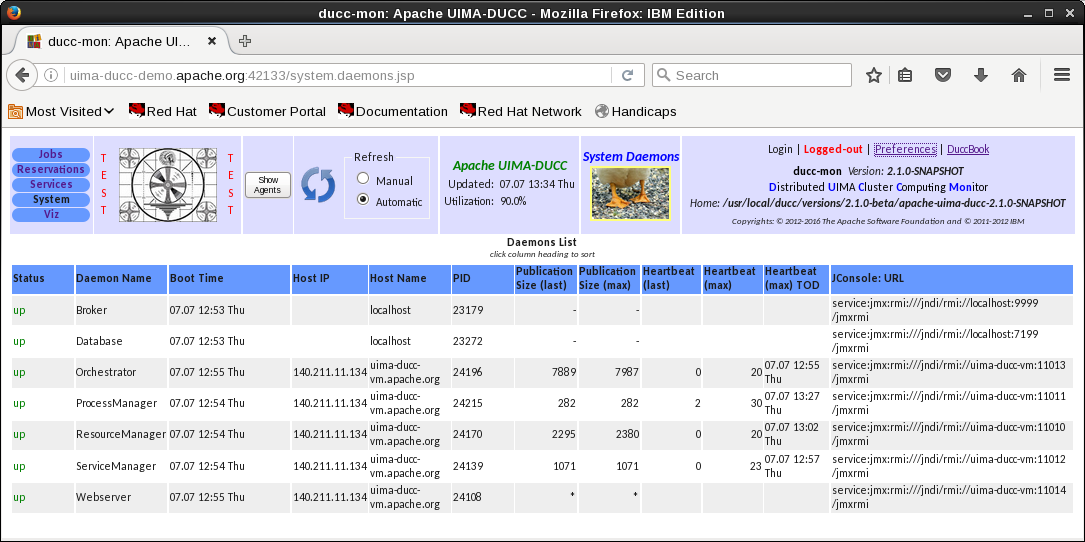
\includegraphics[width=90mm]{images/ducc-webserver/System-Daemons.png}
\caption{Sample Webserver Page}
\end{figure}

    Normally, the Web Server automatically fetches new data from {\DUCC} and updates the display.
    This is controlled by setting one of the two refresh modes:
    \begin{itemize}
      \item Manual refresh.  In this mode, the browser windows are updated only by using the
        browser's refresh button, or the {\DUCC} refresh button to the left in the header of
        each page.
      \item Automatic refresh. In this mode, the browser automatically fetches and displays
        new data.  The rate of refresh is currently fixed and cannot be configured.
    \end{itemize}
    
    There is a behavior difference between refresh and reload.
    \paragraph{Refresh}
    Refresh causes the current data on the page to be updated with the most
    current information in the Webserver's possession.  This is performed
    when the refresh button is clicked.
    \paragraph{Reload}
    Reload occurs when the enter key is pressed.  Reload causes not just the
    data to be updated but rather the entire page is replaced.
    
    Two different table styles are supported:
    \begin{itemize}
      \item Scroll, and
      \item Classic.
    \end{itemize}
    Table styles are switched using the {\em Preferences} link.

    \paragraph{Scroll Mode}  When {\em scroll table style} is the preference, a scroll bar is
    shown to the right, within the main window.  The scroll bar allows scrolling to be restricted to the data
    display, leaving column and {\DUCC} headers in place.  In this mode any column may be sorted
    simply by clicking on it.
    
    With respect to sorting, any specified sort is remembered for refresh
    but forgotten for reload.  Sorting is permitted when either manual
    or automatic refresh mode is selected.
    
    The column sort order is maintained until the page is reloaded.

	Note that not all pages have a scroll version - some only have a classic version.
	
    \paragraph{Classic Mode}  When {\em classic table style} is the preference, the
    main data may extend below the bottom of the page and it will be necessary to use the browser's scroller on the right
    to access it.  The column headers and {\DUCC} header scrolls off when doing this.  Columns
    may be sorted in this mode but it is necessary to first switch to ``Manual'' refresh mode to
    prevent browser refreshes during sorting and display of data. 
    
    With respect to sorting, any specified sort is forgotten for refresh
    and reload.  Sorting is only permitted when manual refresh mode is
    selected.
    
    The column sort order is maintained until the page is refreshed or reloaded.

\begin{figure}[ht!]
\centering
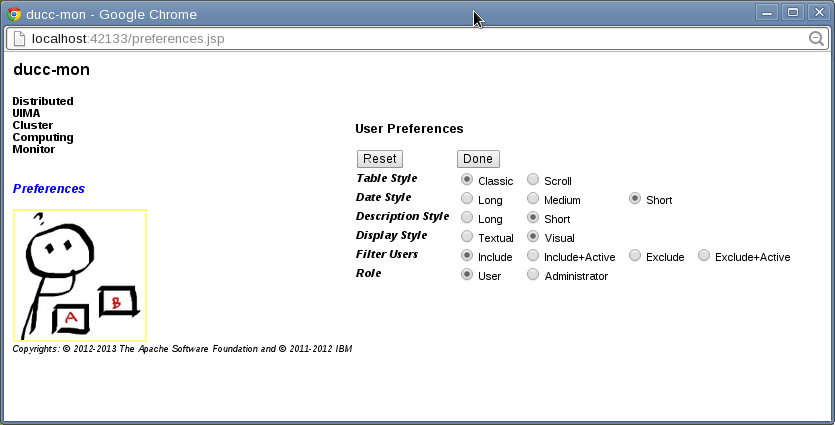
\includegraphics[width=90mm]{images/ducc-webserver/Preferences.png}
\caption{Preferences Page}
\end{figure}

% Create well-known link to this spot for HTML version
\ifpdf
\else
\HCode{<a name='DUCC_WS_COMMON'></a>}
\fi
    \section{Common Links}

        Every page contains a common header containing links and controls. The links permit navigation
        to other content at the site. The controls provide page-wise configuration of the content at
        that page.

        The following links are available on every page of the web server: 

        \begin{description}
          \item[Authentication] \hfill \\ 
            Authentication is needed in order to cancel jobs and reservations, to create a
            reservation, and to perform administration. It is not required to simply view the pages.

            \begin{itemize}
              \item Login - Authenticate and start a session with the Web Server.             
              \item Logout - Terminate the Web Server session 
            \end{itemize}

          \item[Preferences]
            The following preferences may be set:
            \begin{description}
              \item[Table Style] This selects ``scroll'' or ``classic'' display, as
                described above.
              \item[Date Style] This selects long, medium, or long formats for dates.
              \item[Description Style] This selects long or short formats for the various
                description fields.
              \item[Display Style] Choose to display text or (in some circumstances) icons.
              \item[Filter Users] This controls the ``filter'' box near the middle of
                the header on each page.  It allows various levels of inclusion and
                exclusion of active or completed work for the filtered users.
              \item[Role] This allows selection of ``User'' or ``Administrator'' roles.
                This protects registered {\DUCC} administrators from accidentally affecting
                other people's work.
            \end{description}
            
          \item[DuccBook] \hfill \\
            This is a link to the HTML version of the document you are reading.

          \item[Jobs] \hfill \\
            This navigates to the Jobs page, showing all the jobs in the system.

          \item[Reservations] \hfill \\
            This navigates to the Reservations page, showing all the reservations
            in the system and provides a button that can be used to request new reservations. 

          \item[Services] \hfill \\
            This navigates to the Services page, showing all the services in the
            system.

          \item[System] \hfill \\
            This opens a sub-menu with system-related links:
            \begin{itemize}
              \item Administration - This opens a page with administrative functions. 
              \item Broker - This shows information about the AMQ broker employed by the system. 
              \item Classes - This shows all the scheduling classes defined to the system. 
              \item Daemons - This shows the status of {\DUCC}'s management processes. 
              \item DuccBook - This manual. 
              \item Machines - This shows the status of all the {\DUCC} worker nodes. 
            \end{itemize}

            \item[Viz]
            This opens a page with a visualization of the system hosts, showing all
            scheduled work in the system.
      \end{description}              

      % Create well-known link to this spot for HTML version
      \ifpdf
      \else
      \HCode{<a name='DUCC_WS_JOBS'></a>}
      \fi
      % 
% Licensed to the Apache Software Foundation (ASF) under one
% or more contributor license agreements.  See the NOTICE file
% distributed with this work for additional information
% regarding copyright ownership.  The ASF licenses this file
% to you under the Apache License, Version 2.0 (the
% "License"); you may not use this file except in compliance
% with the License.  You may obtain a copy of the License at
% 
%   http://www.apache.org/licenses/LICENSE-2.0
% 
% Unless required by applicable law or agreed to in writing,
% software distributed under the License is distributed on an
% "AS IS" BASIS, WITHOUT WARRANTIES OR CONDITIONS OF ANY
% KIND, either express or implied.  See the License for the
% specific language governing permissions and limitations
% under the License.
% 

    \section{Jobs Page}
    \label{sec:ws.jobs-page}
        The Web Server's home page is also the Jobs page. This page has links to all the rest of the content 
        at the site and shows the status of all the jobs in the system. 
    
        The Jobs page contains the following columns: 

        \begin{description}

            \item[Id] \hfill \\
              This is the ID as assigned by {\DUCC}. This field is hyperlinked to a
              \hyperref[sec:ws-job-details]{Job Details} page for that job that shows the breakdown of
              all the processes assigned to the job and their state.
              
            \item[Start] \hfill \\
              This is the time the Job is accepted into {\DUCC}.
              
            \item[Duration] \hfill \\
              This shows two times.  In green the length of time the job has been running.  In black is
              the estimated time of completion, based on current resources and remaining work.  When
              the job completes, the time shown is the total elapsed time of the job.
                            
            \item[User] \hfill \\
              This is the userid of the job owner.
              
            \item[Class] \hfill \\
              This is the resource class the job is submitted to.
              
            \item[State] \hfill \\
              This shows the state of the job.  The normal job progression is shown below, with an
              explanation of what each state means.
              \begin{description}
                  \item[Received] - The job has been vetted, persisted, and assigned a unique ID. 
                  \item[WaitingForDriver] - The job is waiting for the Job Driver to initialize. 
                  \item[WaitingForServices] - The job is waiting for verification from the
                    Service Manager that required services are started and responding.  This may
                    cause {\DUCC} to start services if necessary.  In that even this state will
                    persist until all pre-requisite services are ready.
                  \item[WaitingForResources] - The job is waiting to be scheduled. In busy
                    systems this may require preemption of existing work.  In that case this
                    state will persist until preemption is complete.
                  \item[Initializing] - The job initializing. Usually this
                    is the UIMA-AS initialization phase.  In the default configuration, only
                    two (2) processes are allocated by the Resource Manager.  No additional
                    resources are allocated until at least one of the new processes successfully
                    completes initialization.  Once initialization is complete the Resource Manager
                    will double the number of allocated processes until the user's fair share of
                    the resources is attained.
                  \item[Running] - At least one process is now initialized and running. 
                  \item[Completing] - The last work item has completed and {\DUCC} is freeing resources.
                    If the job had many resources allocated at the time the job exited this state
                    will persist until all allocated resources are freed.
                  \item[Completed] - The job is complete. 
              \end{description}
                  
            \item[Reason or Extraordinary Status] \hfill \\

              % See this structure:
              % org.apache.uima.ducc.transport.event.common.IDuccCompletionType
              
              This field contains miscellaneous information pertaining to the job.  If the job exits
              the system for any reason, that reason is shown here.  If the job's pre-requisite
              services are unavailable (or ailing) that fact is displayed here.  If there is a
              job monitor running, that fact is shown here.  Most of the values for this field
              support ``hovers'' containing additional information about the reason.
         
              \begin{description}
                  \item[EndOfJob] - The job and completed ran with no errors. 
                  \item[Error] - All work items are processes but at least one had an error. 
                  \item[CanceledByDriver] - The Job Driver (JD) terminated the job. The reason for
                    termination is seen by hovering over the text with your mouse.
                  \item[CanceledBySystem] - The job was canceled because {\DUCC} was shutdown. 
                  \item[CanceledBySser] - The job owner or {\DUCC} administrator canceled the job. 
                  \item[Cancel Pending] - The job has been canceled and is not yet fully evicted
                    from the system.
                  \item[DriverInitializationFailure] - The Job Driver (JD) process is unable to initialize. Hover over 
                    the field with your mouse for details (if any are available), and check your JD log. 
                  \item[DriverProcessFailed] - The Job Driver (JD) process failed for some reason. Hover over the 
                    field with your mouse for details (if any), and check your JD log. 
                  \item[MonitorActive] The job has a console monitor active.  This is enabled with the
                    job's ``wait\_for\_completion'' parameter on job submission.
                  \item[ServicesUnavailable] - The job declared a dependency on one or more services, and the 
                    Service Manager (SM) cannot find or start the required service. 
                  \item[Premature] - The job was terminated for some unknown reason before all work items were 
                    processed. Check the JP logs for details. 
                  \item[ProcessInitializationFailure] - Too many processes failed during
                    initialization and the job was canceled by {\DUCC}.  Check the JP logs for the
                    reason.
                  \item[ProcessFailure] - Too many processes failed while running and {\DUCC} canceled
                    the job.  Check the JP logs for the reason.
                  \item[ResourcesUnavailable] - The Resource Manager (RM) is unable to allocate resources for 
                    the job. For non-preemptable jobs this could be because the limit on that type of allocation is 
                    reached, or all the hosts are already allocated and work cannot be preempted to make space for 
                    it. For all jobs, it could be because the job class is invalid. 
                    \item[{\em service\_name}] If there is a service name in this field it indicates the job is
                      dependent on the service but the service is not responding to the {\DUCC} Service Monitor's
                      pinger.
              \end{description}

            \item[Services] \hfill \\
              This is the number of services the job has declared dependencies on.  There is a ``hover'' that
              shows the ids of the services, if any.

            \item[Processes] \hfill \\
              This is the number of processes currently assigned to the job.

            \item[Init Fails] \hfill \\
              This is the total number of initialization failures experienced by the job. This
              field is hyperlinked to pages with log excerpts highlighting the specific failures.
              
            \item[Run Fails] \hfill \\
              This is the total number of process failures experienced by the job. This field is
              hyperlinked to pages with log excerpts highlighting the specific failures.
              
            \item[PgIn] This is the number of page-in events, over all processes, on the machines
              running the job.

            \item[Swap] This is the total swap space, over all the processes, being used by the job.

            \item[Size] \hfill \\
              This is the declared memory size of the job
              
            \item[Total] \hfill \\
              This is the total number of work items declared by the job.
              
            \item[Done] \hfill \\
              This is the total number of work items successfully completed for the job.
              
            \item[Error] \hfill \\
              This is the total number of exceptions thrown or other errors experienced by work
              items. This field is hyperlinked to pages containing log excerpts highlighting
              the failures.
              
            \item[Dispatch] \hfill \\
              This is the total number CASs that are currently dispatched. 

              This usually represents the quantity derived from the following formula:
\begin{verbatim}              
     min( (initialized.processes * threads.per.process), (incomplete.work.items - errors) )
\end{verbatim}

              The actual number is a measured number, not a calculated number, and may differ
              slightly from the formula if the measurement is taken immediately after process
              start-up, or in the time between a work item completing and a new one being
              dispatched.
              
            \item[Retry] \hfill \\
              This is the number of CASs that were retried for any reason.  Reasons for retry
              include preemption for fair-share, work-item timeout, or error conditions.

              Note: If a work item in any process fails, the entire process is considered
              suspect, and all work-items in the process are terminated.  Work items in the
              process which did not have errors are re-dispatched (retried) to a different
              process.
              
            \item[Preempt] \hfill \\
              This is the total number of processes that have been preempted to make room for
              other work due to Fair Share.
              
            \item[Description] \hfill \\
              This is the description string from the $--$description string from submit.
            \end{description}

    \begin{figure}[ht!]
    \centering
    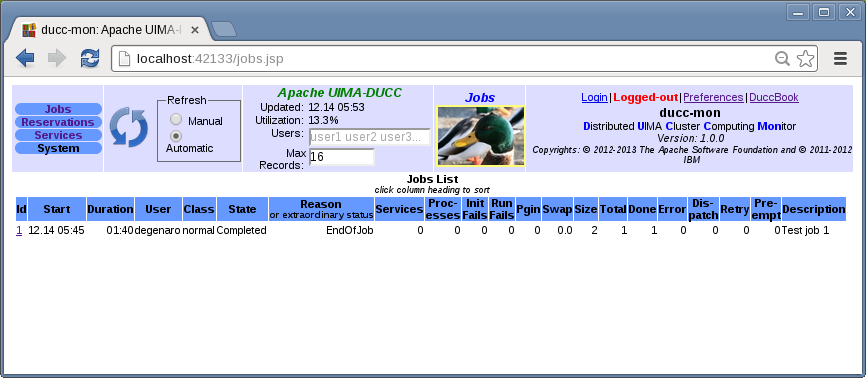
\includegraphics[width=90mm]{images/ducc-webserver/Jobs.png}
    \caption{Jobs Page}
    \end{figure}
            


      % Create well-known link to this spot for HTML version
      \ifpdf
      \else
      \HCode{<a name='DUCC_WS_JOB_DETAILS'></a>}
      \fi
      % 
% Licensed to the Apache Software Foundation (ASF) under one
% or more contributor license agreements.  See the NOTICE file
% distributed with this work for additional information
% regarding copyright ownership.  The ASF licenses this file
% to you under the Apache License, Version 2.0 (the
% "License"); you may not use this file except in compliance
% with the License.  You may obtain a copy of the License at
% 
%   http://www.apache.org/licenses/LICENSE-2.0
% 
% Unless required by applicable law or agreed to in writing,
% software distributed under the License is distributed on an
% "AS IS" BASIS, WITHOUT WARRANTIES OR CONDITIONS OF ANY
% KIND, either express or implied.  See the License for the
% specific language governing permissions and limitations
% under the License.
% 
  
    \section{Job Details Page}
    \label{sec:ws-job-details}

    This page shows details of all the processes that run in support of a job. 
    The information is divided among five tabs:
    \begin{description}
      \item[Processes] This tab contains details on all the processes for the job, both
        active, and defunct.
      \item[Work Items] This tab shows details for each individual work-item in the job.
      \item[Performance] This tab shows a performance break-down of all the UIMA analytics
        in the job.
      \item[Specification] This tab shows the job specification for the job.
      \item[Files] This tab shows the files in the log directory.
      \end{description}
      
    \subsection{Processes}
    \label{subsec:ws-processes}
    The processes page contains the following columns:
    
    \begin{description}

        \item[Id] \hfill \\
          This is the {\DUCC}-assigned numeric id of the process (not the Operating System's
          process Id). Process 0 is always the Job Driver.          

        \item[Log] \hfill \\
          This is the log name for the process. It is hyperlinked to the log itself.

        \item[Log Size] \hfill \\
          This is the size of the log in MB. If you find you have trouble viewing the log
          from the Web Server it could be because it is too big to view in the server and needs to
          be read by some other means than the Web Server.  (It is not currently paged in by 
          the Web Server, it is read in full.)

        \item[Host Name] \hfill \\
          This is the name of the host where the process ran.

        \item[PID] \hfill \\
          This is the Unix process ID (PID) of the process.

        \item[State Scheduler] \hfill \\
          % The information comes from here:
          % State Scheduler: org.apache.uima.ducc.transport.event.common.IResourceState.ResourceState

          This shows the Resource Manager state of the job. It is one of:
          \begin{description}
              \item[Allocated] - The host is currently allocated for this job by the RM.
              \item[Deallocated] - The resource manager has deallocated the shares for the job on
                this host.
          \end{description}

        \item[Reason Scheduler or extraordinary status] \hfill \\
          \phantomsection\label{itm:job-details-sched}


          % The information comes from here:
          % Reason Scheduler: org.apache.uima.ducc.transport.event.common.IResourceState.ProcessDeallocationType
          This column provides a reason for the scheduler state, when the scheduler state is other than ``Allocated''. 
          These may have ``hovers'' that provide more information
          if it is available.

            \begin{description}          
                \item[AutonomousStop] - The process terminated unexpectedly of its own accord ("crashed", or
                  simply exited.) 

                \item[Exception] - The process is terminated by the JD exception handler. 

                \item[Failed] - The process is terminated by the Agent because the JP wrapper was able to detect and 
                  communicate a fatal condition (Exception) in the pipeline.. 
                  
                \item[FailedInitialization] - The process is terminated because the UIMA initialization step failed. 
                  
                \item[Forced] - The host is preempted by RM for other work because of fair share. 
                  
                \item[JobCanceled] - The job was canceled by the user or a system administrator. 
                  
                \item[JobCompleted] - The process is canceled because of {\DUCC} restart. 
                  
                \item[JobFailure] - The job failure limit is exceeded, causing the job to be canceled by the JD.                    
                  
                \item[InitializationTimeout] - The UIMA initialization phase exceeded the configured timeout. 
                  
                \item[Killed] - The agent terminated the process for some reason. The ``Reason Agent'' field
                  should have more details in this case.
          
                \item[Stopped]	- The process was terminated by the Agent for some reason.  The hover should
                  contain more information.
                          
                \item[Voluntary] - The job is winding down, there's no more work for this host, so it stops. 
                  
                \item[Unknown] - None of the above. This is an exceptional condition, sometimes an
                  internal {\DUCC} error. Check the JP and JD logs for possible causes..
            \end{description}

          \item[State Agent] \hfill \\
          \phantomsection\label{itm:job-details-state}

          % This state comes from here:
          % State Agent: org.apache.uima.ducc.transport.event.common.IProcessState.ProcessState
            This shows the {\DUCC} Agent's view of the state of the process.
            \begin{description}
               \item[Starting] The {\DUCC} process manager as issued a request to the assigned {\DUCC} Agent to
                 start the process.
               \item[Initializing] The process is initializing.  Usually this means the UIMA analytic
                 pipeline (Job Process) is executing its initialization method.
              \item[Running] The Job Process has completed the initialization phase and is ready for 
                or actively executing work.
              \item[Stopped] The {\DUCC} Agent reports the process is stopped and (and has exited).
              \item[Failed] The {\DUCC} Agent reports the process failed with errors.  This usually
                means that UIMA-AS has detected exceptions in the pipeline and reported them
                to the Job Driver for logging.
              \item[FailedInitialization] The process died during the UIMA initialization phase.
              \item[InitializationTimeout] The process exceeded the site's limit for time spent
                in UIMA initialization.
              \item[Killed] The {\DUCC} Agent killed the process for some reason.  There are
                three reasons for this:
                \begin{enumerate}
                  \item The Job Processes failed to initialize,
                  \item The Job Process timed out during initialization,
                  \item The process exceeded its allowed swap.
                \end{enumerate}
              \item[Abandoned] It is possible to cancel a specific process of a job.  Usually
                this is because it became ``stuck'' because of hardware failure.  If a process
                is killed in \hyperref[sec:cli.ducc-cancel]{this way}, the state is recorded as {\em Abandoned}.
            \end{description}
            
          \item[Reason Agent] \hfill \\
          \phantomsection\label{itm:job-details-agent}

          This shows extended reason information if a process exited other than having run out
          of work to do.

            \begin{description}
              \item[AgentTimedOutWatingForORState] The {\DUCC} Agent is expecting a state update
                from the {\DUCC} Orchestrator.  Timer on this wait has expired.  This usually 
                indicates an infrastructure or communication problem.
              \item[Croaked] The process exited for no good or clear reason, it simply vanished.
              \item[Discontinued] This is the normal reason when the process is stopped as directed.
              \item[ExceededShareSize] The process exceeded it's declared memory size.
              \item[ExceededSwapThreshold] The process exceeded the configured swap threshold.
              \item[FailedInitialization] The process was terminated because the UIMA 
                initialization step failed.
              \item[InitializationTimeout] The process was terminated because the UIMA initialization
                step took too long.
              \item[JPHasNoActiveJob] This is set when an agent looses connectivity while its
                JPs are running. The job finishes (stopped or killed). The agent regains
                connectivity. The OR publish no longer includes the job but the agent still has
                processes running for that job. The agent kills ghost processes with the reason:
                JPHasNoActiveJob.
              \item[LowSwapSpace] The process was terminated because the system is about to run
                out of swap space.  This is a preemptive measure taken by {\DUCC} to avoid exhaustion
                of swap, to effect orderly eviction of the job before the operating system starts
                its own reaping procedures.
              \item[AdministratorInitiated] The process was canceled by an administrator.
              \item[UserInitated] The process was canceled by the owning user.
            \end{description}
                    
          \item[Exit] \hfill \\
            The process exit code or signal.
            
          \item[Time Init] \hfill \\
            This is the clock time this process spent in initialization.
            
          \item[Time Run] \hfill \\
            This is the clock time this process spent in executing, not including
            initialization.
            
          \item[Time GC] \hfill \\
            This is amount of time spent in Java Garbage Collection for the process.
            
          \item[PgIn] \hfill \\
            This is the number of page-in events on behalf of the process.

          \item[Swap] \hfill \\
            This is the amount of swap space on the machine being consumed by the process.

          \item[\%CPU] \hfill \\
            Current CPU percent consumed by the process.  This will be $>$ 100\% on 
            multi-core systems if more than one core is being used.  Each core contributes
            up to 100\% CPU, so, for example, on a 16-core machine, this can be as high
            as 1600\%.
            
          \item[RSS] \hfill \\
            The amount of real memory being consumed by the process (Resident Storage Size)
            
          \item[Time Avg] \hfill \\
            This is the average time in seconds spent per work item in the process.
            
          \item[Time Max] \hfill \\
            This is the maximum time in seconds spent per work item in the process.
            
          \item[Time Min] \hfill \\
            This is the minimum time in seconds spent per work item in the process.
            
          \item[Done] \hfill \\
            This is the number of work items processed in this process.
            
          \item[Error] \hfill \\
            This is the number of exceptions processing work items in this process.
                      
          \item[Dispatch] \hfill \\
            The number of work items currently dispatched.
              
          \item[Retry] \hfill \\
            This is the number of work items that were retried in this process for any reason, excluding
            preemption.
            
          \item[Preempt] \hfill \\
            This is the number of work items that were preempted from this process, if
            fair-share caused preemption.
            
          \item[JConsole URL] \hfill \\
            This is a URL that can be used to connect via JMX to the processes, e.g. via
            jconsole.

      \end{description}
      
    \begin{figure}[ht!]
    \centering
    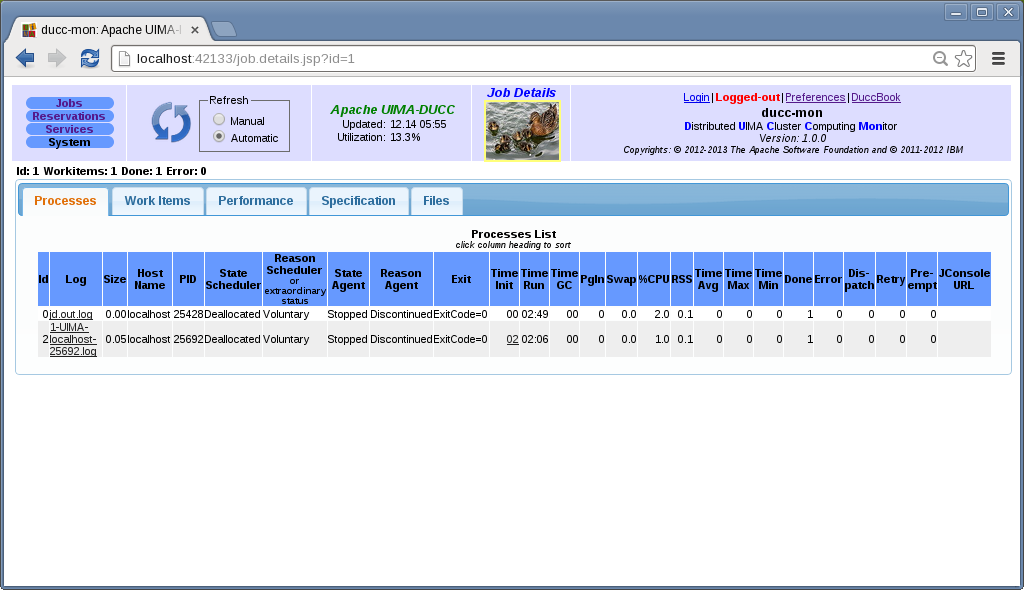
\includegraphics[width=90mm]{images/ducc-webserver/Job-Details-Processes.png}
    \caption{Processes Tab}
    \end{figure}
    
   \subsection{Work Items}
   \label{subsec:ws-work-items}
   This tab provides details for each individual work item.  Columns include:

   % The data comes from here: org.apache.uima.ducc.common.jd.files.IWorkItemState.State    
   \begin{description}
     \item[SeqNo]  \hfill \\
       This is the sequence work items are fetched from the Collection Reader's
       getNext() method by the {\DUCC} Job Driver.
     \item[Id]  \hfill \\
       This is the name of the work item.
     \item[Status]  \hfill \\
       The is the current state of the work item.  
       States include:
       \begin{description}
         \item[ended] The work item is complete.
         \item[error] The work item ended with errors.
         \item[operating] The work item is current being executed.
         \item[retry] The work item is being retried.
         \item[start] The work item has been picked up for execution and {\DUCC} is waiting
           for confirmation that it is running.
       \end{description}
       If a work item has not yet been retrieved from the Collect Reader it does not show
       on this page.
     \item[Delivery Time (sec)]  \hfill \\
       The time spent in getting a work item from the Job Driver to a Job Process.
     \item[Process Time (sec)]  \hfill \\
       The time spent processing the work item.
     \item[Investment Time (sec)]  \hfill \\
       The time spent processing the work item during the current epoch.
     \item[Node (IP)]  \hfill \\
       The host IP where the work item was processed.
     \item[Node (Name)]  \hfill \\
       The host name where the work item was processed.
     \item[PID]  \hfill \\
       The Unix Process Id that the work item was processed in.
   \end{description}
    
    \begin{figure}[ht!]
    \centering
    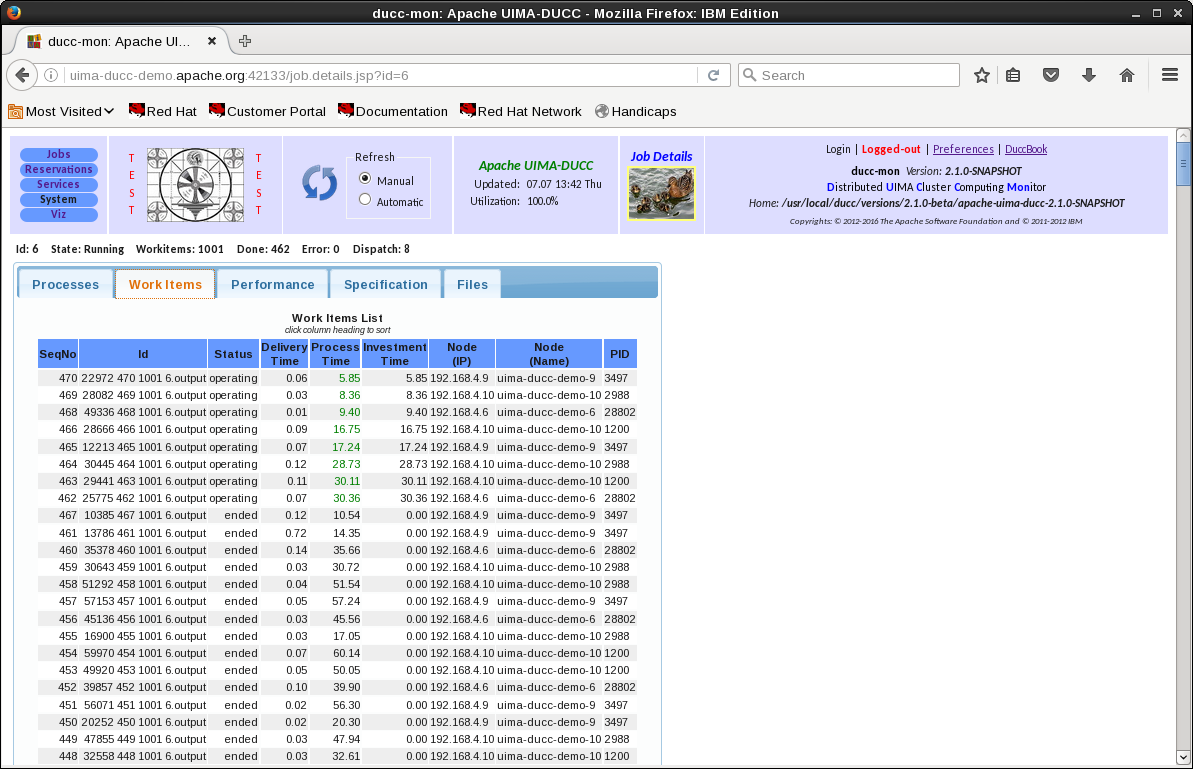
\includegraphics[width=90mm]{images/ducc-webserver/Job-Details-WorkItems.png}
    \caption{Work Items Tab}
    \end{figure}  

   \subsection{Performance}
   \label{subsec:performance}
   This tab shows performance summaries of all the pipeline components.  The statistics
   are aggregated over all instances of each component in each process of the job.
   
   \begin{description}
     \item[Name]  \hfill \\
       The short name of the analytic.
     \item[Total]  \hfill \\
       This is the total time in days, hours, minutes, and seconds taken by each
       component of the pipeline.
     \item[\% of Total]  \hfill \\
       This is the percent of the total usage consumed by this analytic.
     \item[Avg]  \hfill \\
       This is the average time spent by all the instances of the analytic.
     \item[Min]  \hfill \\
       This is the minimum time spent by any instance of the analytic.
     \item[Max]  \hfill \\
       This is the maximum time spent by any instance of the analytic.
   \end{description}
    
    \begin{figure}[ht!]
    \centering
    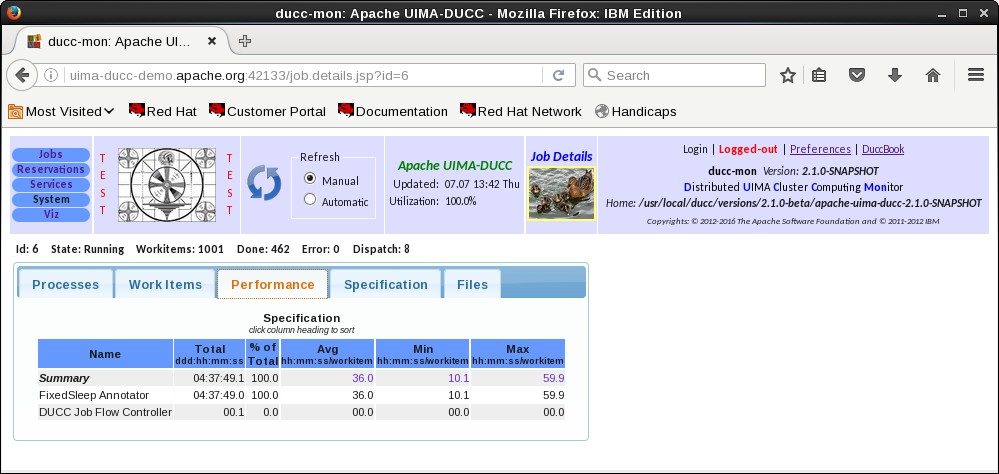
\includegraphics[width=90mm]{images/ducc-webserver/Job-Details-Performance.png}
    \caption{Performance Tab}
    \end{figure}  
       
   \subsection{Specification}
   This tab shows the full job specification in the form of a Java Properties
   file.  This will include all the parameters specified by the user, plus those
   filled in by {\DUCC}.
    
    \begin{figure}[ht!]
    \centering
    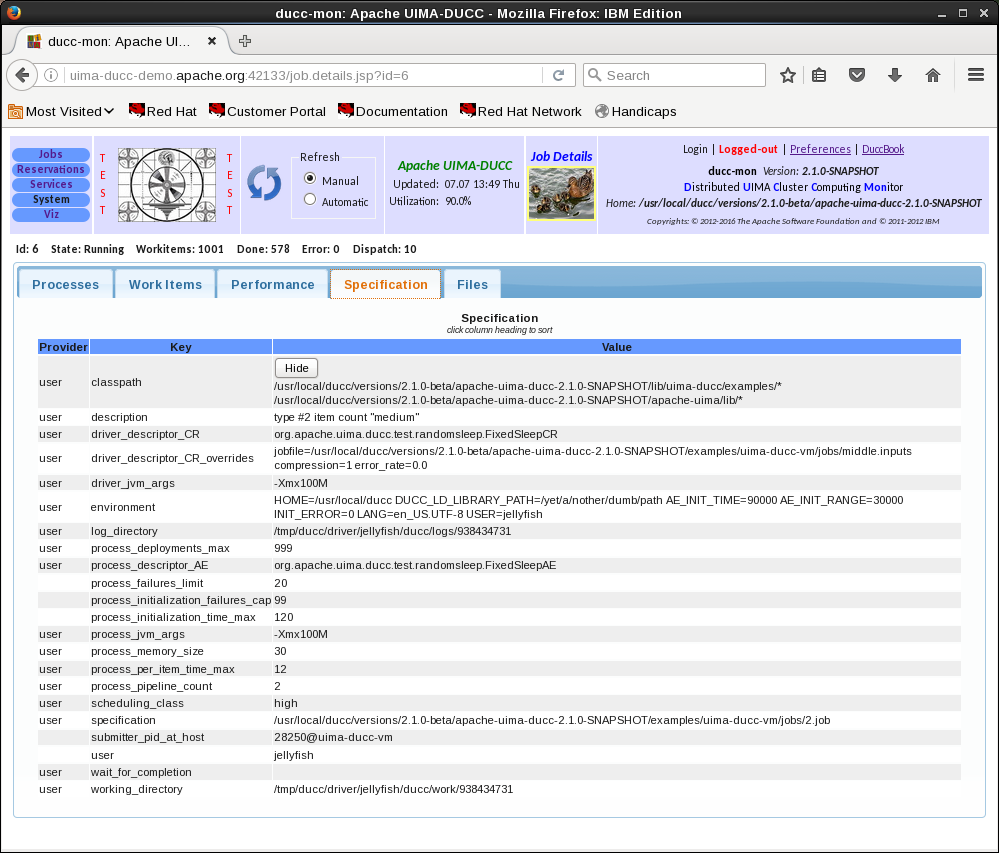
\includegraphics[width=90mm]{images/ducc-webserver/Job-Details-Specification.png}
    \caption{Specification Tab}
    \end{figure}  
    
   \subsection{Files}
   This tab shows the files in the log directory.


      % Create well-known link to this spot for HTML version
      \ifpdf
      \else
      \HCode{<a name='DUCC_WS_RESERVATIONS'></a>}
      \fi
      % 
% Licensed to the Apache Software Foundation (ASF) under one
% or more contributor license agreements.  See the NOTICE file
% distributed with this work for additional information
% regarding copyright ownership.  The ASF licenses this file
% to you under the Apache License, Version 2.0 (the
% "License"); you may not use this file except in compliance
% with the License.  You may obtain a copy of the License at
% 
%   http://www.apache.org/licenses/LICENSE-2.0
% 
% Unless required by applicable law or agreed to in writing,
% software distributed under the License is distributed on an
% "AS IS" BASIS, WITHOUT WARRANTIES OR CONDITIONS OF ANY
% KIND, either express or implied.  See the License for the
% specific language governing permissions and limitations
% under the License.
% 

\section{Reservations Page}
\label{sec:ws-reservations}

This page shows details of all reservations.  There are two types of reservations: {\em managed}
and {\em unmanaged}.

A {\em managed reservation} is a reservation whose process is fully managed by {\DUCC}.  This process
is any arbitrary process and is submitted with the
\hyperref[sec:cli.ducc-process-submit]{ducc\_process\_submit} CLI.  The lifetime of the reservation
starts at the time {\DUCC} assigns a unique ID, and ends when the process terminates for any reason.

An {\em unmanaged reservation} is essentially a sandbox for the user.  {\DUCC} starts no processes
in the reservation and manages none of the processes which run on that host.  The lifetime of the
reservation starts at the time {\DUCC} assigns a unique ID, and ends when the submitter or system
administrator cancels it.

The Reservations page contains the following columns: 
\begin{description}

\item[Id] \hfill \\
  This is the unique {\DUCC} numeric id of the reservation as assigned when the reservation is made.
  If this is a {\em managed} reservation, the ID is hyperlinked to a
  \hyperref[sec:ws-managed-reservation-details]{Managed Reservation Details} page with extended
  details on the process running in the reservation.

\item[Start] \hfill \\
  This is the time the reservation was made.
  
\item[Duration] \hfill \\
  A time in green is the length of time the active reservation has been assigned.  
  A time in black is the length of time the completed reservation was assigned. 
  
\item[User] \hfill \\
  This is the userid that made the reservation.
  
\item[Class] \hfill \\
  This is the scheduling class used to schedule the reservation.
  
\item[Type] \hfill \\
  This is the reservation type, {\em managed} or {\em unmanaged}, as described 
  \hyperref[sec:ws-reservations]{above}.

\item[State] \hfill \\
  % 1. org.apache.uima.ducc.transport.event.common.IDuccState
  This is the status of the reservation. Values include: Received - Reservation
  has been vetted, persisted, and assigned unique Id.
  \begin{description}
  \item[Assigned] - The reservation is active. 
  \item[Completed] - The reservation has been terminated.
  \item[Received] - The Reservation has been vetted, persisted, and assigned a unique ID.
  \item[WaitingForResources] - The reservation is waiting for the Resource Manager to find and 
    schedule resources. 
  \end{description}

\item[Reason] \hfill \\

  % 2. org.apache.uima.ducc.transport.event.common.IDuccCompletionType

  If a reservation is not active, this shows the reason.  Note that for
  {\em unmanaged reservations}, even if the user has processes running in the
  reservation, {\DUCC} does NOT attempt to terminate those processes (hence, ``unmanaged''.)

  For {\em managed reservations}, {\DUCC} does terminate the associated process.

  \begin{description}
  \item[CanceledBySystem] - In the case of the special JobDriver reservation, this is
    canceled by {\DUCC} and reestablished on reboot; hence the state is a result of {\DUCC}
    having been restarted.

    In all other cases, it is a result of {\DUCC} being restarted {\em COLD}.  When
    {\DUCC} is started {\em COLD}, all previous reservations are canceled.  (When {\DUCC}
    is started {\em WARM}, the default, previous reservations are preserved.)
  \item[CanceledByAdmin] - The {\DUCC} administrator released the reservation. 
  \item[CanceledByUser] - The reservation owner released the reservation. 
  \item[ResourcesUnavailable] - The Resource Manager was unable to find free or freeable resources 
    to match the resource request. 
  \item[ProgramExit] - The reservation is a {\em managed} reservation and the associated
    process has exited.
  \end{description}

\item[User Processes] This is the number of processes owned by the user running in the reservation.  
  
  Note that even for {\em unmanaged} reservations, the {\DUCC} agent tracks processes owned
  by the user and reports on them.  This allows better identification and management of
  abandoned reservations.
          
\item[PgIn] This is the number of page-in events for the managed reservation.

\item[Swap] This is the total swap space for the managed reservation.

\item[Memory] \hfill \\
  The memory size in GB of the reservation.  This is the amount of memory that
  was {\em requested}.  In the case of RESERVE policy reservations, that actual memory
  of the reserved machine may be greater.
  
\item[Host Names] \hfill \\
  The host names of the machines where the resources are allocated.
  
\item[Description] \hfill \\
  This is the description string from the --description string from submit.
\end{description}

    \begin{figure}[ht!]
    \centering
    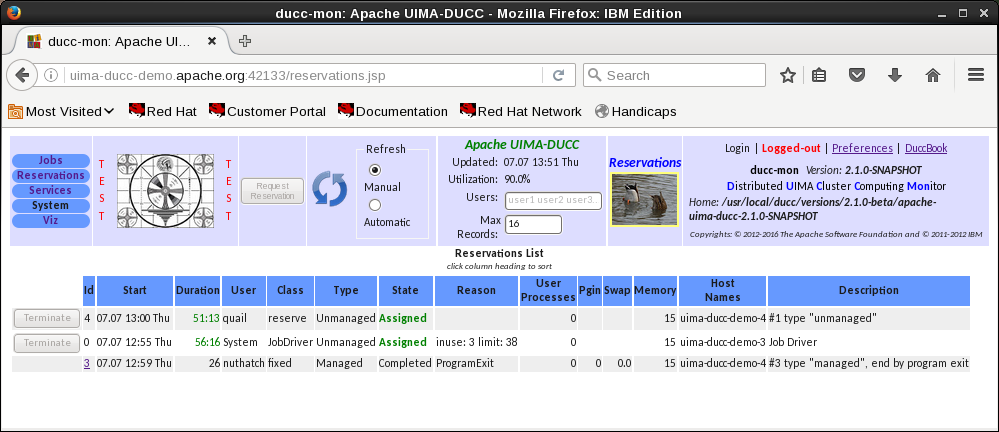
\includegraphics[width=90mm]{images/ducc-webserver/Reservations.png}
    \caption{Reservations Page}
    \end{figure}


      % Create well-known link to this spot for HTML version
      \ifpdf
      \else
      \HCode{<a name='DUCC_WS_RESERVATIONS_DETAILS'></a>}
      \fi
      % 
% Licensed to the Apache Software Foundation (ASF) under one
% or more contributor license agreements.  See the NOTICE file
% distributed with this work for additional information
% regarding copyright ownership.  The ASF licenses this file
% to you under the Apache License, Version 2.0 (the
% "License"); you may not use this file except in compliance
% with the License.  You may obtain a copy of the License at
% 
%   http://www.apache.org/licenses/LICENSE-2.0
% 
% Unless required by applicable law or agreed to in writing,
% software distributed under the License is distributed on an
% "AS IS" BASIS, WITHOUT WARRANTIES OR CONDITIONS OF ANY
% KIND, either express or implied.  See the License for the
% specific language governing permissions and limitations
% under the License.
% 
\section{Managed Reservation Details Page}
\label{sec:ws-managed-reservation-details}

This page shows details of the processes which run in a managed reservation.  The
information is divided between three tabs:

   \begin{description}
       \item[Processes] This tab contains details on all the processes contained in the
         reserved space.
       \item[Specification] This tab shows the specification for the process.
       \item[Files] This tab shows the files in the log directory.
   \end{description}  

   \subsection{Processes}
   \label{sec:ws-manres-processes}

   The processes page contains the following columns:
   \begin{description}
      \item[Id] \hfill \\
        This is the {\DUCC}-assigned numeric id of the process.  This format of this
        id is two numbers:
\begin{verbatim}
    RESID.SHAREID
\end{verbatim}
        Here, the {\em RESID} is the reservation ID.  The {\em SHAREID} is the 
        share ID assigned by the Resource Manager.  Together these form a unique
        ID for each process that runs in the reservation.
        
        Note: The current version of {\DUCC} supports only one process per managed
        reservation.  Future versions are expected to support multiple processes
        within a single managed reservation.
        
      \item[Log] \hfill \\
        This is the log name for the process. It is hyperlinked to the log itself.
        
      \item[Log Size] \hfill \\
        This is the size of the log in MB. If you find you have trouble viewing the log
        from the web server it could be because it is too big to view in the browser.
        
      \item[Host Name] \hfill \\
        This is the name of the host where the process is running (or ran).
        
      \item[PID] \hfill \\
        This is the Unix process ID (PID) of the process.
        
      \item[State Scheduler] \hfill \\
        This shows the Resource Manager state of the job. It is one of:
        
        \begin{description}
            \item[Allocated] - The resource manager has allocated resources for this process on the host.
            \item[Deallocated] - The resource manager has deallocated resources for this process on the host.
        \end{description}
        
      \item[Reason Scheduler or Extraordinary Status] \hfill \\
        These are the same as for the \hyperref[itm:job-details-sched]{job details.}

      \item[State Agent] \hfill \\
        These are the same as for the \hyperref[itm:job-details-state]{job details.}

      \item[Reason Agent] \hfill \\
        These are the same as for the \hyperref[itm:job-details-agent]{job details.}

      \item[Exit] \hfill \\
        The process exit code or signal.

      \item[Time Run] \hfill \\
        The current duration of the reservation, or total duration if it has 
        terminated.
      
      \item[PgIn] \hfill \\
        This is the number of page-in events on behalf of the process.

      \item[Swap] \hfill \\
        This is the amount of swap space on the machine being consumed by the process.
      
      \item[\%CPU] \hfill \\
        Current CPU percent consumed by the process.  This will be $>$ 100\% on 
        multi-core systems if more than one core is being used.  Each core contributes
        up to 100\% CPU, so, for example, on a 16-core machine, this can be as high
        as 1600\%.
      
      \item[RSS] \hfill \\
        The amount of real memory being consumed by the process (Resident Storage Size)

   \end{description}

   \subsection{Specification}
   \label{sec:ws-service-specification}
   This tab shows the full managed reservation specification in the form of a Java Properties
   file.  This will include all the parameters specified by the user, plus those
   filled in by {\DUCC}.
        
   \subsection{Files}
   This tab shows the files in the log directory.
        

      % Create well-known link to this spot for HTML version
      \ifpdf
      \else
      \HCode{<a name='DUCC_WS_SERVICES'></a>}
      \fi
      
    \section{Services Page}
    \label{ws:services-page}
        This page shows details of all services.           

        The Services page contains the following columns: 
        \begin{description}

            \item[Id] \hfill \\
              This is the unique numeric DUCC id of the service.  This ID is hyperlinked to a
              \hyperref[sec:ws-service-details]{Servic Details} page with extended
              details on the service.  Note that for some types of services, DUCC may not
              know more about the service than is shown on the main page.

            \item[Name] \hfill \\
              This is the unique service endpoint of the service.  
              
            \item[Type] \hfill \\
              This is the service type.
              
              There are a number of variants on service types, as discussed in the
              \hyperref[sec:services.types]{services} section of this book.  The webserver
              simplifies these into the following three values:
              \begin{itemize}
                \item Registered
                \item Submitted
                \item Implicit
              \end{itemize}
              
            \item[State] \hfill \\
              This is the state of the service with respect to the service manager.  It is a
              consolidated state over all the service instances.  Valid states are
              \begin{description}
                \item[Available] At least one service instance is responding to the service
                  pinger, indicating it is functional.
                \item[Initializing] No service instances are running but at least one instance
                  is in its UIMA-AS {\em initializing} phase.
                \item[Waiting] At least one service instance is in Running state, and the Service
                  Manager is waiting for a response from the service pinger.
                \item[NotAvailable] No service instance is running. 
                \item[Stopping] The service has been stopped for some reason, but not all 
                  instances have terminated.
              \end{description}

              DUCC will start dependent jobs ONLY if it's services are in state Available.  Otherwise
              DUCC attempts to start the service, and if successful, allows the job to start.  

              If a job is already running and a service becomes other than Available, the
              \hyperref[sec:ws.jobs-page]{jobs page} indicates the service is not available but the job is 
              allowed to continue.
              
            \item[Pinger] \hfill \\
              This indicates whether the Service Manager is running a pinger for the service.
              
            \item[Health] \hfill \\
              {\em Health} is a status returned by each pinger and is the result of that pinger's
              evaluation of the state of the service.  It is shown as on of
              \begin{itemize}
                \item {\em Good}
                \item {\em Bad}
              \end{itemize}
              Both terms are highly subjective.  Pingers may return a summary of the underlying
              data used to label a service as good or bad.  That status is shown as a hover over
              this field.
              
            \item[Instances] \hfill \\
              This is the number of instances (processes) currently registered for the service.  

            \item[Deployments] \hfill \\
              This is the number of actual instances deployed for the service.  Note that this may
              be greater, or less, than the number of registered instances, if the service owner
              decides to temporarily start or stop additional instances.

            \item[User] \hfill \\
              This is the userid of the service owner.
              
            \item[Class] \hfill \\
              This is the scheduling class the service is running in. 
              
              If a service is registered as ``ping-only'', no resources are allocated for it.  This
              is shown as a class of {\tt ping-only}.
              
            \item[Size] \hfill \\
              This is the memory size, in GB, of each service instance

            \item[Jobs] \hfill \\
              This is the number of jobs currently using the service.  The IDs of the jobs are
              shown as hovers over this field.

            \item[Services] \hfill \\
              Services may themselves depend on other services.  This field shows the number of
              services dependent on this service.  The dependent service IDs are shown with a 
              hover over the field.

            \item[Reservations] \hfill \\
              This field shows the number of
              managed reservations dependent on this service. The IDs of the managed reservations
              rea shown as a hover over the field.

              
            \item[Description] \hfill \\
              This is the description string from the --description string from submit.
        \end{description}


      % Create well-known link to this spot for HTML version
      \ifpdf
      \else
      \HCode{<a name='DUCC_WS_SERVICE_DETAILS'></a>}
      \fi
      % 
% Licensed to the Apache Software Foundation (ASF) under one
% or more contributor license agreements.  See the NOTICE file
% distributed with this work for additional information
% regarding copyright ownership.  The ASF licenses this file
% to you under the Apache License, Version 2.0 (the
% "License"); you may not use this file except in compliance
% with the License.  You may obtain a copy of the License at
% 
%   http://www.apache.org/licenses/LICENSE-2.0
% 
% Unless required by applicable law or agreed to in writing,
% software distributed under the License is distributed on an
% "AS IS" BASIS, WITHOUT WARRANTIES OR CONDITIONS OF ANY
% KIND, either express or implied.  See the License for the
% specific language governing permissions and limitations
% under the License.
% 
\section{Service Details Page}
\label{sec:ws-service-details}

This page shows details of the processes which implement. 

The information is divided between four tabs:

   \begin{description}
       \item[Deployments] This tab contains details on all the processes implementing
         the service, if any.
       \item[Registry] This tab shows the registration information for the service.
       \item[Files] This tab shows the files in the log directory. 
       \item[History] This tab contains details on all the completed processes implementing the service, if any.  
   \end{description}  

   \subsection{Deployments}
   \label{sec:ws-services-processes}

   The deployments page contains the following columns:
   \begin{description}
      \item[Id] \hfill \\
        This is the {\DUCC}-assigned numeric id of the process.  This format of this
        id is two numbers:
\begin{verbatim}
    RESID.SHAREID
\end{verbatim}
        Here, the {\em RESID} is the Orchestrator assigned instance ID.  The {\em SHAREID} is the 
        instance ID assigned by the Resource Manager.  Together these form a unique
        ID for each process that runs in the service.
               
      \item[State] \hfill \\
        The state of this service instance.
               
      \item[Services] \hfill \\
        The current state of service dependencies.
                                
      \item[Log] \hfill \\
        This is the log name for the process. It is hyperlinked to the log itself.
        
      \item[Log Size] \hfill \\
        This is the size of the log in MB. If you find you have trouble viewing the log
        from the web server it could be because it is too big to view in the browser.
        
      \item[Host Name] \hfill \\
        This is the name of the node where the process is running (or ran).
        
      \item[PID] \hfill \\
        This is the Unix process ID (PID) of the process.
       
      \item[Memory] \hfill \\
        The service process actual memory size (GB).
                
      \item[State Scheduler] \hfill \\
        This shows the Resource Manager state of the service instance. It is one of:
        
        \begin{description}
            \item[Allocated] - The node is still allocated for this service instance by the RM.
            \item[Deallocated] - The resource manager has deallocated the resources for the service instance on
              this node.
        \end{description}
        
      \item[Reason Scheduler or Extraordinary Status] \hfill \\
        These are the same as for the \hyperref[itm:job-details-sched]{job details.}

      \item[State Agent] \hfill \\
        These are the same as for the \hyperref[itm:job-details-state]{job details.}

      \item[Reason Agent] \hfill \\
        These are the same as for the \hyperref[itm:job-details-agent]{job details.}

      \item[Exit] \hfill \\
        The process exit code or signal.

      \item[Time Init] \hfill \\
        Most services are UIMA-AS services and therefore have an {\em initialization} phase
        to their lifetimes.  This field shows the time spent in that phase.

      \item[Time Run] \hfill \\
        The current duration of the instance, or total duration if it has 
        terminated.
        
      \item[Time GC] \hfill \\
        This is amount of time spent in Java Garbage Collection for the process.

      \item[Pgin] \hfill \\
        This is the number of page-in events on behalf of the process.
        
      \item[Swap] \hfill \\
        This is the amount of swap space on the machine being consumed by the process.
        
      \item[\%CPU] \hfill \\
        Current CPU percent consumed by the process.  This will be $>$ 100\% on 
        multi-core systems if more than one core is being used.  Each core contributes
        up to 100\% CPU, so, for example, on a 16-core machine, this can be as high
        as 1600\%.

      \item[RSS] \hfill \\
        The amount of real memory being consumed by the process (Resident Storage Size)

      \item[JConsole URL] \hfill \\
        This is a URL that can be used to connect via JMX to the processes, e.g. via
        jconsole.

   \end{description}

   \subsection{Registry}
   \label{sec:ws-managed-reservation-specification}
   This tab shows the full service specification in the form of a Java Properties
   file.  This will include all the parameters specified by the user, plus those
   filled in by {\DUCC}.
        
   The registry for a Service contains two types of entries:
   \begin{enumerate}
     \item Service specification properties, prefixed with ``svc''. These comprise
       the service specification that the Service Manager submits on behalf of
       a user in order to start registered services.
     \item Meta properties, prefixed with ``meta''.  This is the Service Manager's state
       record for the service as it is running.  In addition to state it contains
       properties required for service registration that are not used for
       service submission.
   \end{enumerate}
           
   \subsection{Files}
   This tab shows the files in the log directory.
   
           
   \subsection{History}
   This tab shows the completed service instances.
   


      % Create well-known link to this spot for HTML version
      \ifpdf
      \else
      \HCode{<a name='DUCC_WS_SYSTEM'></a>}
      \fi
      % 
% Licensed to the Apache Software Foundation (ASF) under one
% or more contributor license agreements.  See the NOTICE file
% distributed with this work for additional information
% regarding copyright ownership.  The ASF licenses this file
% to you under the Apache License, Version 2.0 (the
% "License"); you may not use this file except in compliance
% with the License.  You may obtain a copy of the License at
% 
%   http://www.apache.org/licenses/LICENSE-2.0
% 
% Unless required by applicable law or agreed to in writing,
% software distributed under the License is distributed on an
% "AS IS" BASIS, WITHOUT WARRANTIES OR CONDITIONS OF ANY
% KIND, either express or implied.  See the License for the
% specific language governing permissions and limitations
% under the License.
% 

\section{System Pages}
\label{sec:system-details}

These pages show information relating to the {\DUCC} System itself:
\begin{description}
  \item[Administration]This displays system administrators and implements
    the interface to various administrative controls.
  \item[Broker] This shows selective information for the system's broker.
  \item[Classes] This shows the system's scheduling class definitions.
  \item[Daemons] This shows the status of all {\DUCC} processes.
  \item[DuccBook] This is a link to the book you are reading.
  \item[Machines] This shows details of all the machines (nodes) in the {\DUCC} cluster.
\end{description}

\subsection{Administration}

   This page has two tabs:
   \begin{description}   
     \item[Administrators] This shows the user-ids that are authorized to administer
       {\DUCC}.  In addition to executing the ``Control'' functions described below,
       administrators may cancel any job, reservation, or service, and may modify
       services they do not own.  

       In order to perform administrative functions, the following must be satisfied:
       \begin{enumerate}
         \item The user is logged-in to the web server.
         \item The user is a registered administrator.
         \item The user has set the role as ``administrator'' in the {\DUCC} Preferences
           page.  This is a safeguard so that administrators who are also users
           are less likely to inadvertently affect other people's jobs.
       \end{enumerate}
     \item[Control] Currently {\DUCC} supports a single administrative control function
       via the web server: Stop new job submissions and re-enable them.  If submissions
       are blocked, all existing work runs normally, but no new work is accepted.
     \end{description}


\subsection{Broker}
This page shows selective information for the system's broker.
Information includes host, port, version, uptime, memory used, threads, load average, topics and queues.

\subsection{Classes}
This page shows the definitions of the {\DUCC} scheduling classes.  The scheduling classes are
discussed in more detail in the \hyperref[sec:rm.job-classes]{Resource Manager} section.

\subsection{Daemons}
\label{sec:system-details.daemons}

This page shows the current state of all {\DUCC} processes.  By default, only the administrative
processes, Broker, Database, Orchestrator, ProcessManager, ResourceManager, ServiceManager, and Webserver are
shown.  A button in the upper left of the page titled ``Show Agents'' enables display of
the status of all the {\DUCC} agents as well. (Agents are suppressed by default because the
page is expensive to render for large systems.)

The columns shown on this page include

   \begin{description}
      \item[Status] \hfill \\
        This indicates whether the daemon is running and broadcasting state {\em up},
        or not {\em down}.  
        
        All {\DUCC} daemons broadcast a heartbeat containing process state.  If the Status
        is {\em down}, either the daemon is not functioning, or something is preventing
        state from reaching the web server via {\DUCC}'s ActiveMQ instance.

      \item[Daemon Name] \hfill \\
        This is the name of the process.

      \item[Boot Time] \hfill \\ 
        This shows the date and time of the latest boot of the specific process.
          
      \item[Host IP] \hfill \\ 
        This is the IP address of the processor where the process is running.

      \item[Host Name] \hfill \\ 
        This shows the hostname of the processor where the process is running.

      \item[PID] \hfill \\ 
        This is the Unix process Id of the {\DUCC} process.

      \item[Publication Size (last)] \hfill \\ 
        This shows the size of the most recent state publication of the process, in bytes.

      \item[Publication Size (max)] \hfill \\ 
        This shows the size of the largest state publication of the process, in bytes.

      \item[Heartbeat (last)] \hfill \\ 
        This shows the number of seconds since the last state publication for the process. 
         Large numbers here indicate potential cluster or {\DUCC} problems.

      \item[Heartbeat (max)] \hfill \\ 
        This shows the longest delay since a state publication for the process was received
        at the web server.  Large numbers here indicate potential cluster or {\DUCC} problems.

      \item[Heartbeat (max) TOD] \hfill \\ 
        This shows the time the longest delay of a state publication occurred.

      \item[JConsole URL] \hfill \\ 
        This is the jconsole URL for the process.

   \end{description}
      
\subsection{Machines}

This page shows the states of all the machines (nodes) in the {\DUCC} cluster.

The columns shown on this page include

   \begin{description}
      \item[Status] \hfill \\
        This shows the current state of a machine.  Values include:
        \begin{description}
          \item[defined] The node is in the {\DUCC}
            \hyperref[sec:admin-ducc.nodes]{nodes file}, but no {\DUCC} process has been
            started there, or else there is a communication problem and
            the state messages are not being delivered.
            \item[up] The node has a {\DUCC} Agent process running on it and the
              resource manager is receiving regular heartbeat packets from it.
            \item[down] The node had a healthy {\DUCC} Agent on it at some point
              in the past (since the last {\DUCC} boot), but the resource manager
              has stopped receiving heartbeats from it. 

              The agent may have been manually shut down, may have crashed, or there
              may be a communication problem.

              Additionally, very heavy loads from jobs running the the node can cause
              the {\DUCC} Agents heartbeats to be delayed.
        \end{description}

      \item[IP] \hfill \\
        This is the IP address of the node.


      \item[Name] \hfill \\
        This is the hostname of the node.

      \item[Nodepool] \hfill \\
        This is the host nodepool.

      \item[Memory(GB) usable] \hfill \\
        This is the amount of usable memory, in GB, as reported by each machine.  
        This is the maximum amount that can be allocated by the resource manager.
        
        Usually the amount will be slightly less than the installed memory.  This is because
        a small bit of memory is usually reserved by the hardware for its own purposes.  For 
        example, a machine with 48GB of installed memory may report only 47GB available.

      \item[Memory(GB) free] \hfill \\
        This is the amount of free memory, in GB, as reported by each machine.
        This is the amount not presently allocated by the resource manager.
        
      \item[CPU] \hfill \\
        This is the host CPU one minute load average.
        
      \item[Swap(GB) inuse] \hfill \\
        This is the total size in-use swap data.  {\DUCC} shows any value greater than 0 in
        red as swapping can very significantly slow applications.  However, swap use does
        not always mean there is a performance problem.  This is flagged by {\DUCC} simply
        as an alert of a potential problem

      \item[Swap(GB) free] \hfill \\
        This is the total size of swap area.  

      \item[C-Groups] \hfill \\
        If on then C-Groups are in use and processes deployed by {\DUCC} will
        be limited in resource consumption.


      \item[Alien PIDs] \hfill \\
        This shows the number of processes not owned by {\DUCC}, the operating system, or
        jobs scheduled on each node.  The Unix Process IDS of these processes is displayed
        in a hover.

        {\DUCC} preconfigures many of the standard operating 
        \hyperref[itm:props-rogue.process]{system process} and 
        \hyperref[itm:props-rogue.user]{userids}.  This list may be updated by each
        installation.

        A common cause of alien PIDs is errant process run in unmanaged reservations.  A
        user may reserve a machine for use as a sandbox.  If the reservation is released
        without properly terminating all the processes, they may linger.  When {\DUCC} 
        schedules the node for other purposes, significant performance penalties may be
        paid due to competition between the legitimately scheduled work and the leftover
        ``alien'' processes.  The purpose of this column is to bring attention to this situation.


      \item[Heartbeat(last)] \hfill \\
        This shows the number of seconds since the last agent heartbeat from this machine.

      \end{description}
      


      % Create well-known link to this spot for HTML version
      \ifpdf
      \else
      \HCode{<a name='DUCC_WS_Viz'></a>}
      \fi
      % 
% Licensed to the Apache Software Foundation (ASF) under one
% or more contributor license agreements.  See the NOTICE file
% distributed with this work for additional information
% regarding copyright ownership.  The ASF licenses this file
% to you under the Apache License, Version 2.0 (the
% "License"); you may not use this file except in compliance
% with the License.  You may obtain a copy of the License at
% 
%   http://www.apache.org/licenses/LICENSE-2.0
% 
% Unless required by applicable law or agreed to in writing,
% software distributed under the License is distributed on an
% "AS IS" BASIS, WITHOUT WARRANTIES OR CONDITIONS OF ANY
% KIND, either express or implied.  See the License for the
% specific language governing permissions and limitations
% under the License.
% 

    \section{Visualization}
    \label{sec:ws.vizualization}
       This page shows a visualization of all scheduled work.  Every host is represented by a square
       whose area is proportional to the amount of memory on the host.  If work is scheduled to a
       host, it is represented by a rectangle whose area is proportional to the amount of memory
       that is scheduled for the work.  In a multi-user environment, each userid is mapped into 
       a different color, making it possible to see the usage per-user.

       Hovers are provided to show the real memory size of each host, the schedulable memory for
       each host, and the amount of memory scheduled for each bit of work.

       If multiple allocations are made on a single host for the same job or service, the rectangles
       are combined into a single rectangle, reducing clutter and better showing the actual usage
       of the job (or service).   

       Clicking on any box representing scheduled work sends the browser to the details page for 
       the corresponding work.

       The screenshot below shows a visualization with a handful of 127GB hosts, 48GB hosts, and
       32GB hosts.  Regular UIMA-AS jobs show as untextured boxes; for example, job 6080, owned
       by user Hilaria, running in a 37GB allocation in host bluej291-41 which is a 127GB host.

       Hosts bluej291-45 and 291-46 are running Managed Reservations, which are shown with
       crosshatches from lower-left to upper right.

       Hosts bluej291-37 and bluej291-40 are running Unmanaged Reservations, shown with
       vertical-horizontal crosshatches.

       Below bluej291-34, bluej291-36, bluej293-49, and bluej293-60 are running {\DUCC}-managed
       services, shown by crosshatching from upper-left to lower-right.

       The host representations may be sorted by clicking on the ``size'' or the ``name'' text
       near the top of the display.


           \begin{figure}[ht!]
    \centering
    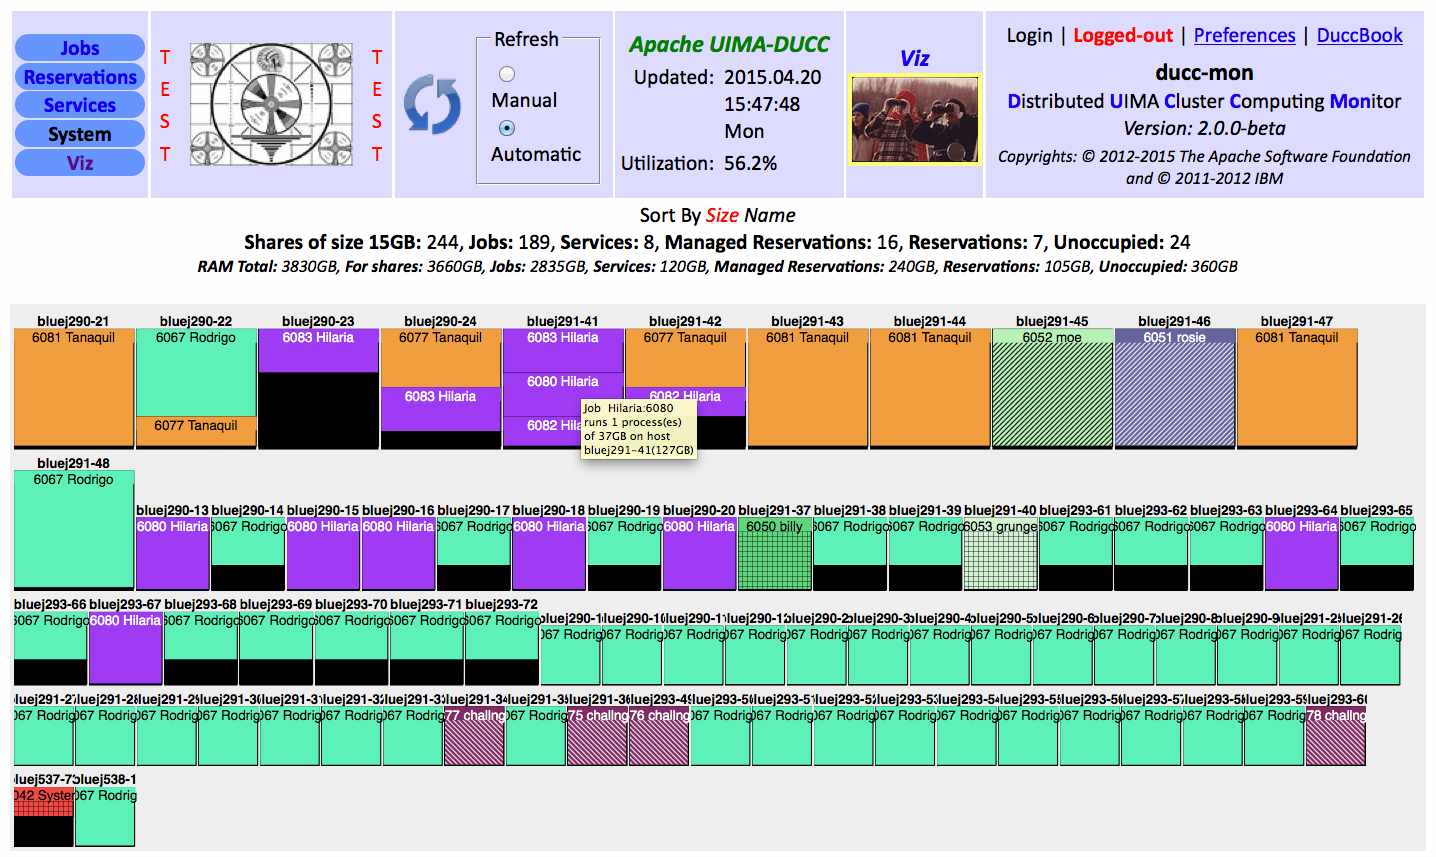
\includegraphics[width=160mm]{images/ducc-webserver/viz.jpg}
    \caption{Visualization}
    \end{figure}




